\documentclass[spanish,]{book}
\usepackage{lmodern}
\usepackage{amssymb,amsmath}
\usepackage{ifxetex,ifluatex}
\usepackage{fixltx2e} % provides \textsubscript
\ifnum 0\ifxetex 1\fi\ifluatex 1\fi=0 % if pdftex
  \usepackage[T1]{fontenc}
  \usepackage[utf8]{inputenc}
\else % if luatex or xelatex
  \ifxetex
    \usepackage{mathspec}
  \else
    \usepackage{fontspec}
  \fi
  \defaultfontfeatures{Ligatures=TeX,Scale=MatchLowercase}
\fi
% use upquote if available, for straight quotes in verbatim environments
\IfFileExists{upquote.sty}{\usepackage{upquote}}{}
% use microtype if available
\IfFileExists{microtype.sty}{%
\usepackage{microtype}
\UseMicrotypeSet[protrusion]{basicmath} % disable protrusion for tt fonts
}{}
\usepackage{hyperref}
\hypersetup{unicode=true,
            pdftitle={Introducción al Análisis de Datos},
            pdfauthor={Matías Alfonso},
            pdfborder={0 0 0},
            breaklinks=true}
\urlstyle{same}  % don't use monospace font for urls
\ifnum 0\ifxetex 1\fi\ifluatex 1\fi=0 % if pdftex
  \usepackage[shorthands=off,main=spanish]{babel}
\else
  \usepackage{polyglossia}
  \setmainlanguage[]{spanish}
\fi
\usepackage{natbib}
\bibliographystyle{apalike}
\usepackage{color}
\usepackage{fancyvrb}
\newcommand{\VerbBar}{|}
\newcommand{\VERB}{\Verb[commandchars=\\\{\}]}
\DefineVerbatimEnvironment{Highlighting}{Verbatim}{commandchars=\\\{\}}
% Add ',fontsize=\small' for more characters per line
\usepackage{framed}
\definecolor{shadecolor}{RGB}{248,248,248}
\newenvironment{Shaded}{\begin{snugshade}}{\end{snugshade}}
\newcommand{\KeywordTok}[1]{\textcolor[rgb]{0.13,0.29,0.53}{\textbf{#1}}}
\newcommand{\DataTypeTok}[1]{\textcolor[rgb]{0.13,0.29,0.53}{#1}}
\newcommand{\DecValTok}[1]{\textcolor[rgb]{0.00,0.00,0.81}{#1}}
\newcommand{\BaseNTok}[1]{\textcolor[rgb]{0.00,0.00,0.81}{#1}}
\newcommand{\FloatTok}[1]{\textcolor[rgb]{0.00,0.00,0.81}{#1}}
\newcommand{\ConstantTok}[1]{\textcolor[rgb]{0.00,0.00,0.00}{#1}}
\newcommand{\CharTok}[1]{\textcolor[rgb]{0.31,0.60,0.02}{#1}}
\newcommand{\SpecialCharTok}[1]{\textcolor[rgb]{0.00,0.00,0.00}{#1}}
\newcommand{\StringTok}[1]{\textcolor[rgb]{0.31,0.60,0.02}{#1}}
\newcommand{\VerbatimStringTok}[1]{\textcolor[rgb]{0.31,0.60,0.02}{#1}}
\newcommand{\SpecialStringTok}[1]{\textcolor[rgb]{0.31,0.60,0.02}{#1}}
\newcommand{\ImportTok}[1]{#1}
\newcommand{\CommentTok}[1]{\textcolor[rgb]{0.56,0.35,0.01}{\textit{#1}}}
\newcommand{\DocumentationTok}[1]{\textcolor[rgb]{0.56,0.35,0.01}{\textbf{\textit{#1}}}}
\newcommand{\AnnotationTok}[1]{\textcolor[rgb]{0.56,0.35,0.01}{\textbf{\textit{#1}}}}
\newcommand{\CommentVarTok}[1]{\textcolor[rgb]{0.56,0.35,0.01}{\textbf{\textit{#1}}}}
\newcommand{\OtherTok}[1]{\textcolor[rgb]{0.56,0.35,0.01}{#1}}
\newcommand{\FunctionTok}[1]{\textcolor[rgb]{0.00,0.00,0.00}{#1}}
\newcommand{\VariableTok}[1]{\textcolor[rgb]{0.00,0.00,0.00}{#1}}
\newcommand{\ControlFlowTok}[1]{\textcolor[rgb]{0.13,0.29,0.53}{\textbf{#1}}}
\newcommand{\OperatorTok}[1]{\textcolor[rgb]{0.81,0.36,0.00}{\textbf{#1}}}
\newcommand{\BuiltInTok}[1]{#1}
\newcommand{\ExtensionTok}[1]{#1}
\newcommand{\PreprocessorTok}[1]{\textcolor[rgb]{0.56,0.35,0.01}{\textit{#1}}}
\newcommand{\AttributeTok}[1]{\textcolor[rgb]{0.77,0.63,0.00}{#1}}
\newcommand{\RegionMarkerTok}[1]{#1}
\newcommand{\InformationTok}[1]{\textcolor[rgb]{0.56,0.35,0.01}{\textbf{\textit{#1}}}}
\newcommand{\WarningTok}[1]{\textcolor[rgb]{0.56,0.35,0.01}{\textbf{\textit{#1}}}}
\newcommand{\AlertTok}[1]{\textcolor[rgb]{0.94,0.16,0.16}{#1}}
\newcommand{\ErrorTok}[1]{\textcolor[rgb]{0.64,0.00,0.00}{\textbf{#1}}}
\newcommand{\NormalTok}[1]{#1}
\usepackage{longtable,booktabs}
\usepackage{graphicx,grffile}
\makeatletter
\def\maxwidth{\ifdim\Gin@nat@width>\linewidth\linewidth\else\Gin@nat@width\fi}
\def\maxheight{\ifdim\Gin@nat@height>\textheight\textheight\else\Gin@nat@height\fi}
\makeatother
% Scale images if necessary, so that they will not overflow the page
% margins by default, and it is still possible to overwrite the defaults
% using explicit options in \includegraphics[width, height, ...]{}
\setkeys{Gin}{width=\maxwidth,height=\maxheight,keepaspectratio}
\IfFileExists{parskip.sty}{%
\usepackage{parskip}
}{% else
\setlength{\parindent}{0pt}
\setlength{\parskip}{6pt plus 2pt minus 1pt}
}
\setlength{\emergencystretch}{3em}  % prevent overfull lines
\providecommand{\tightlist}{%
  \setlength{\itemsep}{0pt}\setlength{\parskip}{0pt}}
\setcounter{secnumdepth}{5}
% Redefines (sub)paragraphs to behave more like sections
\ifx\paragraph\undefined\else
\let\oldparagraph\paragraph
\renewcommand{\paragraph}[1]{\oldparagraph{#1}\mbox{}}
\fi
\ifx\subparagraph\undefined\else
\let\oldsubparagraph\subparagraph
\renewcommand{\subparagraph}[1]{\oldsubparagraph{#1}\mbox{}}
\fi

%%% Use protect on footnotes to avoid problems with footnotes in titles
\let\rmarkdownfootnote\footnote%
\def\footnote{\protect\rmarkdownfootnote}

%%% Change title format to be more compact
\usepackage{titling}

% Create subtitle command for use in maketitle
\providecommand{\subtitle}[1]{
  \posttitle{
    \begin{center}\large#1\end{center}
    }
}

\setlength{\droptitle}{-2em}

  \title{Introducción al Análisis de Datos}
    \pretitle{\vspace{\droptitle}\centering\huge}
  \posttitle{\par}
    \author{Matías Alfonso}
    \preauthor{\centering\large\emph}
  \postauthor{\par}
      \predate{\centering\large\emph}
  \postdate{\par}
    \date{2019-10-30}

\usepackage{booktabs}
\usepackage{amsthm}
\makeatletter
\def\thm@space@setup{%
  \thm@preskip=8pt plus 2pt minus 4pt
  \thm@postskip=\thm@preskip
}
\makeatother
\usepackage{booktabs}
\usepackage{longtable}
\usepackage{array}
\usepackage{multirow}
\usepackage{wrapfig}
\usepackage{float}
\usepackage{colortbl}
\usepackage{pdflscape}
\usepackage{tabu}
\usepackage{threeparttable}
\usepackage{threeparttablex}
\usepackage[normalem]{ulem}
\usepackage{makecell}
\usepackage{xcolor}

\begin{document}
\maketitle

{
\setcounter{tocdepth}{1}
\tableofcontents
}
\part{Programación en R}\label{part-programacion-en-r}

\chapter{Preliminares}\label{prelim}

R es un lenguaje de programación desarrollado inicialmente por Ross
Ihaka y Robert Gentleman en el departamento de Estadística de la
Universidad de Auckland en 1993. Está orientado específicamente con un
enfoque al análisis estadístico.\\
R se desarrolla a partir de un lenguaje denominado S, desarrollado por
John Chambers en 1976, disponible a partir del software comercial
S-PLUS.\\
Es un lenguaje interactivo, permite la ejecución de instrucciónes en
líneas de comando en una consola.

\section{¿Por qué R?}\label{por-que-r}

R puede ser ejecutado en múltiples plataformas y en la gran mayoría de
los sistemas operativos. Puede ser ejecutado en tablets, teléfonos o
computadoras. La utilización de scripts permite compartir fácilmente los
análisis con los colegas, así como asegurar la reproductibilidad de los
resultados. Todo lo que realizamos mediante una interfaz gráfica con el
mouse no deja registros de nuestro trabajo e impide que podamos repasar
nuestro trabajo para corregir errores.\\
La versatilidad y la potencia que otorga un lenguaje de programación es
mucho mayor que la que podemos obtener con softwares estadísticos de
interfaz gráfica.\\
La comunidad de usuarios y desarrolladores de R está en constante
crecimiento en los últimos años. Hay una enorme cantidad de gente
realizando nuevos desarrollos en R cada día, que están a la vanguardia
de la ciencia computacional y estadística.

\section{Software Libre}\label{software-libre}

La mayor ventaja que tiene R con respecto a otros softwares de análisis
estadístico es que es un software libre. ¿Qué quiere decir eso? Por un
lado, que es gratuito. Por otro, que el código fuente con el que R fue
desarrollado está abierto, se puede descargar y está diponible online.
Actualmente el copyrigth de R lo posee la
\href{https://www.r-project.org/foundation/}{R Foundation}. R forma
parte del \href{https://es.wikipedia.org/wiki/GNU}{sistema GNU},
desarrollado por la
\href{https://es.wikipedia.org/wiki/Free_Software_Foundation}{Free
Software Foundation}. De acuerdo a la Free Software Foundation, con el
software libre se garantizan cuatro libertades fundamentales:

\begin{itemize}
\tightlist
\item
  La libertad de ejecutar el programa para cualquier propósito.
  (Libertad 0)
\item
  La libertad de estudiar cómo el programa funciona y adaptarlo a tus
  propias necesidades. (Libertad 1)
\item
  La libertad de redistribuir copias de manera que puedas ayudar a
  alguien. (Libertad 2)
\item
  La libertad de mejorar el programa, y liberar tus mejoras al público,
  de manera que se beneficie toda la comunidad. (Libertad 3)
\end{itemize}

\section{Sistema de Paquetes}\label{sistema-de-paquetes}

El sistema de funcionalidades de R se encuentra agrupado en paquetes. La
mayor parte de los paquetes se encuentran disponibles en
\href{https://cran.r-project.org/}{Comprehensive R Archive Network
(CRAN)}. Hay un conjunto de paquetes principales, de base, que incluye
todos los paquetes que se instalan por defecto cuando instalamos R.
Luego, tenemos un montón de paquetes con funcionalidades específicas que
podemos instalar en función de nuestras necesidades.

\chapter{Primeros pasos}\label{primeros-pasos}

\section{Asignación de datos y
evaluación.}\label{asignacion-de-datos-y-evaluacion.}

R es un \emph{lenguaje interpretado}. Esto quiere decir que le podemos
ir pasando instrucciones y el programama las irá interpretando. Cuando
ejecutamos el programa, nos encontramos con el prompt a la espera de
intrucciones:

\begin{verbatim}
>
\end{verbatim}

Una de las operaciones más sencillas que podemos realizar es la
asignación de valores a las variables. El operador de asignación es
\texttt{\textless{}-}.

\begin{Shaded}
\begin{Highlighting}[]
\NormalTok{x <-}\StringTok{ }\DecValTok{1}
\KeywordTok{print}\NormalTok{(x)}
\end{Highlighting}
\end{Shaded}

\begin{verbatim}
## [1] 1
\end{verbatim}

\begin{Shaded}
\begin{Highlighting}[]
\NormalTok{x}
\end{Highlighting}
\end{Shaded}

\begin{verbatim}
## [1] 1
\end{verbatim}

\begin{Shaded}
\begin{Highlighting}[]
\NormalTok{texto <-}\StringTok{ "hola mundo"}
\NormalTok{texto}
\end{Highlighting}
\end{Shaded}

\begin{verbatim}
## [1] "hola mundo"
\end{verbatim}

Podemos imprimir el valor de una variable con la función
\texttt{print()} o directamente escribiendo la variable.

Tenemos dos formas de interactuar con R:

\begin{itemize}
\tightlist
\item
  Tipear directamente los comandos en el prompt y ejecutarlos.
\item
  Escribir un archivo de texto con todas las intrucciones y luego
  ejecutarlo. Este archivo se denomina script.
\end{itemize}

\section{Working directory}\label{working-directory}

Lo primero que debemos hacer cuando comenzamos a trabajar en R es
configurar el directorio de trabajo. Una buena costumbre es crear un
directorio nuevo de trabajo cuando comenzamos un proyecto nuevo. Luego
configuramos esa carpeta como directorio de trabajo. Colocamos allí
todos los archivos vinculados a ese proyecto. Para determinar en qué
directorio estamos parados, podemos utilizar el comando
\texttt{getwd()}. Para configurar el directorio de trabajo, utilizamos

\begin{verbatim}
setwd(#RUTA-A-DIRECTORIO)
\end{verbatim}

\section{Comentarios}\label{comentarios}

Todo lo que escribamos luego de un \texttt{\#} en una intrucción, no
será evaluado.

\begin{Shaded}
\begin{Highlighting}[]
\NormalTok{x <-}\StringTok{ }\KeywordTok{c}\NormalTok{(}\DecValTok{3}\NormalTok{, }\DecValTok{4}\NormalTok{, }\DecValTok{5}\NormalTok{)}
\NormalTok{## Esto no se ejecuta}

\NormalTok{x}
\end{Highlighting}
\end{Shaded}

\begin{verbatim}
## [1] 3 4 5
\end{verbatim}

Ello nos permite comentar el código que escribimos, a manera de
documentación.

\section{Objetos básicos en R}\label{objetos-basicos-en-r}

Casi todo lo que encontremos en R, se denominan \emph{objetos}. Hay 5
tipos de objetos básicos o atómicos:

\begin{itemize}
\tightlist
\item
  lógico
\item
  numérico
\item
  entero
\item
  complejo
\item
  caracter
\end{itemize}

Veamos algunos ejemplos:

\begin{Shaded}
\begin{Highlighting}[]
\NormalTok{## Logico}
\OtherTok{TRUE}
\end{Highlighting}
\end{Shaded}

\begin{verbatim}
## [1] TRUE
\end{verbatim}

\begin{Shaded}
\begin{Highlighting}[]
\OtherTok{FALSE}
\end{Highlighting}
\end{Shaded}

\begin{verbatim}
## [1] FALSE
\end{verbatim}

\begin{Shaded}
\begin{Highlighting}[]
\NormalTok{## Numérico}
\KeywordTok{c}\NormalTok{(}\FloatTok{1.509}\NormalTok{, }\FloatTok{2.859}\NormalTok{)}
\end{Highlighting}
\end{Shaded}

\begin{verbatim}
## [1] 1.509 2.859
\end{verbatim}

\begin{Shaded}
\begin{Highlighting}[]
\NormalTok{## Enteros}
\DecValTok{1}\OperatorTok{:}\DecValTok{10}
\end{Highlighting}
\end{Shaded}

\begin{verbatim}
##  [1]  1  2  3  4  5  6  7  8  9 10
\end{verbatim}

\begin{Shaded}
\begin{Highlighting}[]
\NormalTok{## Caracter}
\StringTok{"casa"}
\end{Highlighting}
\end{Shaded}

\begin{verbatim}
## [1] "casa"
\end{verbatim}

Existen muchos más clases de objetos en R. Para averiguar de que tipo es
un objeto, podemos utilizar la función \texttt{class()}

\begin{Shaded}
\begin{Highlighting}[]
\NormalTok{x <-}\StringTok{ }\DecValTok{1}\OperatorTok{:}\DecValTok{10}
\KeywordTok{class}\NormalTok{(x)}
\end{Highlighting}
\end{Shaded}

\begin{verbatim}
## [1] "integer"
\end{verbatim}

\begin{Shaded}
\begin{Highlighting}[]
\KeywordTok{class}\NormalTok{(}\StringTok{"TRUE"}\NormalTok{)}
\end{Highlighting}
\end{Shaded}

\begin{verbatim}
## [1] "character"
\end{verbatim}

Para preguntar por la clase de un objeto, podemos utilizar el comando
\texttt{class()}

\begin{Shaded}
\begin{Highlighting}[]
\NormalTok{x <-}\StringTok{ }\DecValTok{1}\OperatorTok{:}\DecValTok{10}
\KeywordTok{class}\NormalTok{(x)}
\end{Highlighting}
\end{Shaded}

\begin{verbatim}
## [1] "integer"
\end{verbatim}

\begin{Shaded}
\begin{Highlighting}[]
\NormalTok{y <-}\StringTok{ "casa"}
\KeywordTok{class}\NormalTok{(y)}
\end{Highlighting}
\end{Shaded}

\begin{verbatim}
## [1] "character"
\end{verbatim}

\section{Factores}\label{factores}

Los factores son básicamente objetos de clase entero, pero con
etiquetas. Son datos categóricos y pueden estar ordenados o no.

\begin{Shaded}
\begin{Highlighting}[]
\NormalTok{f <-}\StringTok{ }\KeywordTok{factor}\NormalTok{(}\KeywordTok{c}\NormalTok{(}\StringTok{"si"}\NormalTok{, }\StringTok{"si"}\NormalTok{, }\StringTok{"no"}\NormalTok{, }\StringTok{"si"}\NormalTok{))}
\NormalTok{f}
\end{Highlighting}
\end{Shaded}

\begin{verbatim}
## [1] si si no si
## Levels: no si
\end{verbatim}

\begin{Shaded}
\begin{Highlighting}[]
\NormalTok{f <-}\StringTok{ }\KeywordTok{factor}\NormalTok{(}\KeywordTok{c}\NormalTok{(}\StringTok{"bajo"}\NormalTok{, }\StringTok{"bajo"}\NormalTok{, }\StringTok{"medio"}\NormalTok{, }\StringTok{"alto"}\NormalTok{),}
            \DataTypeTok{levels =} \KeywordTok{c}\NormalTok{(}\StringTok{"bajo"}\NormalTok{, }\StringTok{"medio"}\NormalTok{, }\StringTok{"alto"}\NormalTok{),}
            \DataTypeTok{ordered =} \OtherTok{TRUE}\NormalTok{)}
\NormalTok{f}
\end{Highlighting}
\end{Shaded}

\begin{verbatim}
## [1] bajo  bajo  medio alto 
## Levels: bajo < medio < alto
\end{verbatim}

\section{Cómo buscar ayuda}\label{como-buscar-ayuda}

R tiene un sistema de ayuda integrado. Si queremos saber para qué sirve
un comando determinado o como pasarle los argumentos, podemos utilizar
\texttt{?} o \texttt{help()}. Supongamos que queremos saber cómo se
utiliza la función \texttt{sum()}

\begin{Shaded}
\begin{Highlighting}[]
\KeywordTok{help}\NormalTok{(sum)}

\NormalTok{?vector}
\end{Highlighting}
\end{Shaded}

\chapter{Estructuras de datos}\label{estructuras-de-datos}

\section{Vectores}\label{vectores}

La forma más elemental de almacenar datos en R es en un vector. Un
\textbf{vector} es una concatenación de objetos del mismo tipo. Podemos
utilizar la función \texttt{c()} para crear vectores.

\begin{Shaded}
\begin{Highlighting}[]
\NormalTok{x <-}\StringTok{ }\KeywordTok{c}\NormalTok{(}\DecValTok{1}\NormalTok{, }\DecValTok{2}\NormalTok{, }\DecValTok{3}\NormalTok{, }\FloatTok{2.5}\NormalTok{)}
\NormalTok{x <-}\StringTok{ }\KeywordTok{c}\NormalTok{(}\OtherTok{TRUE}\NormalTok{, }\OtherTok{FALSE}\NormalTok{)}
\NormalTok{x <-}\StringTok{ }\KeywordTok{c}\NormalTok{(T, F)}
\NormalTok{x <-}\StringTok{ }\KeywordTok{c}\NormalTok{(}\StringTok{"casa"}\NormalTok{, }\StringTok{"árbol"}\NormalTok{, }\StringTok{"patio"}\NormalTok{)}

\NormalTok{## También podemos utilizar la función vector.}
\NormalTok{x <-}\StringTok{ }\KeywordTok{vector}\NormalTok{(}\DataTypeTok{mode =} \StringTok{"numeric"}\NormalTok{, }\DataTypeTok{length =} \DecValTok{10}\NormalTok{)}
\end{Highlighting}
\end{Shaded}

Si concatenamos elementos de diferente clase, R realizará una coerción
automática de la clase de los objetos.

\begin{Shaded}
\begin{Highlighting}[]
\NormalTok{x <-}\StringTok{ }\KeywordTok{c}\NormalTok{(}\StringTok{"casa"}\NormalTok{, }\DecValTok{2}\NormalTok{) ## character}
\NormalTok{x <-}\StringTok{ }\KeywordTok{c}\NormalTok{(}\OtherTok{TRUE}\NormalTok{, }\DecValTok{2}\NormalTok{) ## numeric}

\KeywordTok{class}\NormalTok{(x)}
\end{Highlighting}
\end{Shaded}

\begin{verbatim}
## [1] "numeric"
\end{verbatim}

\section{Listas}\label{listas}

Las listas también son una concatenación de elementos, pero pueden
contener elementos de diferente clase. Para crear una lista, podemos
utilizar \texttt{list()}

\begin{Shaded}
\begin{Highlighting}[]
\NormalTok{x <-}\StringTok{ }\KeywordTok{list}\NormalTok{(}\StringTok{"peso"}\NormalTok{, }\DecValTok{2}\NormalTok{, }\StringTok{"altura"}\NormalTok{, }\DecValTok{3}\NormalTok{, }\OtherTok{TRUE}\NormalTok{)}
\NormalTok{x}
\end{Highlighting}
\end{Shaded}

\begin{verbatim}
## [[1]]
## [1] "peso"
## 
## [[2]]
## [1] 2
## 
## [[3]]
## [1] "altura"
## 
## [[4]]
## [1] 3
## 
## [[5]]
## [1] TRUE
\end{verbatim}

\section{Matrices}\label{matrices}

Las matrices son vectores, pero con un atributo de dimensión. La
dimensión en sí es un vector de enteros de largo 2.

\begin{Shaded}
\begin{Highlighting}[]
\NormalTok{m <-}\StringTok{ }\KeywordTok{matrix}\NormalTok{(}\DecValTok{1}\OperatorTok{:}\DecValTok{9}\NormalTok{, }\DataTypeTok{nrow =} \DecValTok{3}\NormalTok{)}
\NormalTok{m}
\end{Highlighting}
\end{Shaded}

\begin{verbatim}
##      [,1] [,2] [,3]
## [1,]    1    4    7
## [2,]    2    5    8
## [3,]    3    6    9
\end{verbatim}

\begin{Shaded}
\begin{Highlighting}[]
\KeywordTok{dim}\NormalTok{(m)}
\end{Highlighting}
\end{Shaded}

\begin{verbatim}
## [1] 3 3
\end{verbatim}

Al igual que los vectores, contienen objetos de la misma clase. Las
matrices tienen algunas propiedades matemáticas interesantes, pues se
pueden realizar operaciones especiales con ellas, por ejemplo, se pueden
sumar o multiplicar.

\section{Data frames}\label{data-frames}

Los data frames son datos tabulados. Son tablas, donde cada columna
puede ser de una clase diferente. Es un objeto particularmente útil para
el análisis estadístico.

\begin{Shaded}
\begin{Highlighting}[]
\KeywordTok{data.frame}\NormalTok{(}\DataTypeTok{Id =} \KeywordTok{c}\NormalTok{(}\DecValTok{1}\NormalTok{, }\DecValTok{2}\NormalTok{, }\DecValTok{3}\NormalTok{),}
           \DataTypeTok{Nombre =} \KeywordTok{c}\NormalTok{(}\StringTok{"Juan"}\NormalTok{, }\StringTok{"Carlos"}\NormalTok{, }\StringTok{"Ramona"}\NormalTok{),}
           \DataTypeTok{Altura =} \KeywordTok{c}\NormalTok{(}\FloatTok{1.76}\NormalTok{, }\FloatTok{1.80}\NormalTok{, }\FloatTok{1.65}\NormalTok{))}
\end{Highlighting}
\end{Shaded}

\begin{verbatim}
##   Id Nombre Altura
## 1  1   Juan   1.76
## 2  2 Carlos   1.80
## 3  3 Ramona   1.65
\end{verbatim}

\section{Valores faltantes}\label{valores-faltantes}

Existen dos tipos de valores faltantes en R:

\begin{itemize}
\tightlist
\item
  \texttt{NA}
\item
  \texttt{NaN}
\end{itemize}

\chapter{Obteniendo datos}\label{obteniendo-datos}

Existen una enorme cantidad de funciones para abrir archivos de diversos
tipos.

\section{Datos tabulares}\label{datos-tabulares}

Un formato estándar y abierto para guardar información en forma de
tablas son archivos separados por comas (.csv) Para leer estos datos
podemos utilizar:

\begin{itemize}
\tightlist
\item
  \texttt{read.tables()}
\item
  \texttt{read.csv()}
\end{itemize}

Podemos descargar la base de datos del Titanic del siguiente link
\href{../data/titanic.csv}{titanic.csv}. Descargamos y colocamos el
archivo en una carpeta \texttt{data}, dentro del directorio de trabajo:

\begin{Shaded}
\begin{Highlighting}[]
\NormalTok{## Leemos los datos desde un archivo y los guardamos en la variable base}
\NormalTok{base <-}\StringTok{ }\KeywordTok{read.csv}\NormalTok{(}\StringTok{"data/titanic.csv"}\NormalTok{)}

\NormalTok{## Imprimimos las primeras 5 filas de la base}
\KeywordTok{head}\NormalTok{(base)[, }\DecValTok{1}\OperatorTok{:}\DecValTok{3}\NormalTok{]}
\end{Highlighting}
\end{Shaded}

\begin{verbatim}
##   PassengerId Survived Pclass
## 1           1        0      3
## 2           2        1      1
## 3           3        1      3
## 4           4        1      1
## 5           5        0      3
## 6           6        0      3
\end{verbatim}

También podemos leer datos directamente de la web

\begin{Shaded}
\begin{Highlighting}[]
\NormalTok{## Datos Abiertos}
\NormalTok{## Cantidad de consultas médicas y odontológicas en centros de Salud del Primer nivel 2003 - 2019.}
\NormalTok{consultas <-}\StringTok{ }\KeywordTok{read.csv}\NormalTok{(}\StringTok{"http://datos.salud.gob.ar/dataset/5fcacd04-58eb-4b43-89a0-55231c58f1b4/resource/ed9e418f-9858-44df-8ce7-a74fde738684/download/consultas-medicamentos-esenciales.csv"}\NormalTok{)}


\KeywordTok{head}\NormalTok{(consultas)}
\end{Highlighting}
\end{Shaded}

\begin{verbatim}
##   provincia_id                  provincia_desc      año consultas_cantidad
## 1            2 Ciudad Autonoma de Buenos Aires año_2003             559785
## 2            6                    Buenos Aires año_2003            9544395
## 3           10                       Catamarca año_2003             372199
## 4           14                         Cordoba año_2003            3491961
## 5           18                      Corrientes año_2003             764887
## 6           22                           Chaco año_2003            1476825
\end{verbatim}

\begin{Shaded}
\begin{Highlighting}[]
\NormalTok{## Recetas de medicamentos escenciales 2003-2019}
\NormalTok{recetas <-}\StringTok{ }\KeywordTok{read.csv}\NormalTok{(}\StringTok{"http://datos.salud.gob.ar/dataset/dff3bf69-3514-42a3-a2aa-041495895ab2/resource/3b1a2d9e-ac15-484c-aacf-3f3ce79729af/download/recetas-medicamentos-esenciales.csv"}\NormalTok{)}
\end{Highlighting}
\end{Shaded}

\subsection{Excel}\label{excel}

Podemos leer archivos Excel importando la librería \texttt{readxl}

\begin{Shaded}
\begin{Highlighting}[]
\KeywordTok{library}\NormalTok{(readxl)}

\NormalTok{## Excel}
\NormalTok{memoria <-}\StringTok{ }\KeywordTok{read_xls}\NormalTok{(}\StringTok{"./data/EXP1.xls"}\NormalTok{)}

\KeywordTok{head}\NormalTok{(memoria)[}\DecValTok{1}\OperatorTok{:}\DecValTok{3}\NormalTok{]}
\end{Highlighting}
\end{Shaded}

\begin{verbatim}
## # A tibble: 6 x 3
##   Sujeto  NPD1  NPD2
##    <dbl> <dbl> <dbl>
## 1      1    17    16
## 2      4     9    10
## 3      7    11    15
## 4     10    13    14
## 5     13    11    17
## 6     16    12    16
\end{verbatim}

\chapter{Operaciones básicas}\label{operaciones-basicas}

\section{Subsetting. Selección de
elementos.}\label{subsetting.-seleccion-de-elementos.}

Podemos seleccionar elementos o subconjuntos específicos de un objeto de
R. Hay diferentes operadores: \texttt{{[}}, \texttt{{[}{[}}, \texttt{\$}

\subsection{Vectores}\label{vectores-1}

\begin{Shaded}
\begin{Highlighting}[]
\NormalTok{## Creamos un vector con las primeras 10 letras del abecedario.}
\NormalTok{letras <-}\StringTok{ }\NormalTok{letters[}\DecValTok{1}\OperatorTok{:}\DecValTok{10}\NormalTok{]}
\NormalTok{letras}
\end{Highlighting}
\end{Shaded}

\begin{verbatim}
##  [1] "a" "b" "c" "d" "e" "f" "g" "h" "i" "j"
\end{verbatim}

\begin{Shaded}
\begin{Highlighting}[]
\NormalTok{## Por posición}
\NormalTok{letras[}\DecValTok{2}\NormalTok{]}
\end{Highlighting}
\end{Shaded}

\begin{verbatim}
## [1] "b"
\end{verbatim}

\begin{Shaded}
\begin{Highlighting}[]
\NormalTok{letras[}\DecValTok{2}\OperatorTok{:}\DecValTok{3}\NormalTok{]}
\end{Highlighting}
\end{Shaded}

\begin{verbatim}
## [1] "b" "c"
\end{verbatim}

Si los elementos están etiquetados, podemos recuperar los elementos del
vector por sus nombres.

\begin{Shaded}
\begin{Highlighting}[]
\NormalTok{peso <-}\StringTok{ }\KeywordTok{c}\NormalTok{(}\DataTypeTok{Juan =} \DecValTok{70}\NormalTok{, }\DataTypeTok{Pedro =} \DecValTok{85}\NormalTok{, }\DataTypeTok{Ramona =} \DecValTok{65}\NormalTok{)}
\NormalTok{peso[}\StringTok{"Juan"}\NormalTok{]}
\end{Highlighting}
\end{Shaded}

\begin{verbatim}
## Juan 
##   70
\end{verbatim}

\begin{Shaded}
\begin{Highlighting}[]
\NormalTok{peso[}\KeywordTok{c}\NormalTok{(}\StringTok{"Juan"}\NormalTok{, }\StringTok{"Ramona"}\NormalTok{)]}
\end{Highlighting}
\end{Shaded}

\begin{verbatim}
##   Juan Ramona 
##     70     65
\end{verbatim}

También podemos utilizar un vector lógico para recuperar elementos de un
vector.

\begin{Shaded}
\begin{Highlighting}[]
\NormalTok{condicion <-}\StringTok{ }\NormalTok{peso }\OperatorTok{>}\StringTok{ }\DecValTok{68}
\NormalTok{condicion}
\end{Highlighting}
\end{Shaded}

\begin{verbatim}
##   Juan  Pedro Ramona 
##   TRUE   TRUE  FALSE
\end{verbatim}

\begin{Shaded}
\begin{Highlighting}[]
\NormalTok{peso[condicion]}
\end{Highlighting}
\end{Shaded}

\begin{verbatim}
##  Juan Pedro 
##    70    85
\end{verbatim}

\subsection{Matrices}\label{matrices-1}

\begin{Shaded}
\begin{Highlighting}[]
\NormalTok{matriz <-}\StringTok{ }\KeywordTok{matrix}\NormalTok{(letters[}\DecValTok{1}\OperatorTok{:}\DecValTok{9}\NormalTok{], }\DataTypeTok{nrow =} \DecValTok{3}\NormalTok{)}

\NormalTok{## Indicamos el índice de fila y columna.}
\NormalTok{matriz[}\DecValTok{1}\NormalTok{, }\DecValTok{2}\NormalTok{]}
\end{Highlighting}
\end{Shaded}

\begin{verbatim}
## [1] "d"
\end{verbatim}

\begin{Shaded}
\begin{Highlighting}[]
\NormalTok{matriz[}\DecValTok{2}\OperatorTok{:}\DecValTok{3}\NormalTok{, }\DecValTok{1}\OperatorTok{:}\DecValTok{2}\NormalTok{]}
\end{Highlighting}
\end{Shaded}

\begin{verbatim}
##      [,1] [,2]
## [1,] "b"  "e" 
## [2,] "c"  "f"
\end{verbatim}

\subsection{Listas}\label{listas-1}

\begin{Shaded}
\begin{Highlighting}[]
\NormalTok{lista <-}\StringTok{ }\KeywordTok{list}\NormalTok{(}\DataTypeTok{Nombre =} \KeywordTok{c}\NormalTok{(}\StringTok{"Juan"}\NormalTok{, }\StringTok{"Pedro"}\NormalTok{, }\StringTok{"Ramona"}\NormalTok{),}
              \DataTypeTok{Peso =} \KeywordTok{c}\NormalTok{(}\DecValTok{70}\NormalTok{, }\DecValTok{85}\NormalTok{, }\DecValTok{65}\NormalTok{),}
              \DataTypeTok{Altura =} \KeywordTok{c}\NormalTok{(}\FloatTok{1.70}\NormalTok{, }\FloatTok{1.78}\NormalTok{, }\FloatTok{1.65}\NormalTok{))}


\NormalTok{## Podemos recuperar los elementos por posición o por nombre}

\NormalTok{## Devuelve un objeto lista}
\NormalTok{lista[}\DecValTok{1}\NormalTok{]}
\end{Highlighting}
\end{Shaded}

\begin{verbatim}
## $Nombre
## [1] "Juan"   "Pedro"  "Ramona"
\end{verbatim}

\begin{Shaded}
\begin{Highlighting}[]
\NormalTok{lista[}\StringTok{"Nombre"}\NormalTok{]}
\end{Highlighting}
\end{Shaded}

\begin{verbatim}
## $Nombre
## [1] "Juan"   "Pedro"  "Ramona"
\end{verbatim}

\begin{Shaded}
\begin{Highlighting}[]
\NormalTok{## Devuelve la clase del objeto seleccionado}
\NormalTok{lista[[}\DecValTok{1}\NormalTok{]]}
\end{Highlighting}
\end{Shaded}

\begin{verbatim}
## [1] "Juan"   "Pedro"  "Ramona"
\end{verbatim}

\begin{Shaded}
\begin{Highlighting}[]
\NormalTok{lista[[}\StringTok{"Nombre"}\NormalTok{]]}
\end{Highlighting}
\end{Shaded}

\begin{verbatim}
## [1] "Juan"   "Pedro"  "Ramona"
\end{verbatim}

\begin{Shaded}
\begin{Highlighting}[]
\NormalTok{lista}\OperatorTok{$}\NormalTok{Nombre}
\end{Highlighting}
\end{Shaded}

\begin{verbatim}
## [1] "Juan"   "Pedro"  "Ramona"
\end{verbatim}

\subsection{Data frames}\label{data-frames-1}

\begin{Shaded}
\begin{Highlighting}[]
\NormalTok{df <-}\StringTok{ }\KeywordTok{as.data.frame}\NormalTok{(lista)}
\NormalTok{df}
\end{Highlighting}
\end{Shaded}

\begin{verbatim}
##   Nombre Peso Altura
## 1   Juan   70   1.70
## 2  Pedro   85   1.78
## 3 Ramona   65   1.65
\end{verbatim}

\begin{Shaded}
\begin{Highlighting}[]
\NormalTok{df[}\DecValTok{1}\NormalTok{,]}
\end{Highlighting}
\end{Shaded}

\begin{verbatim}
##   Nombre Peso Altura
## 1   Juan   70    1.7
\end{verbatim}

\begin{Shaded}
\begin{Highlighting}[]
\NormalTok{df[,}\DecValTok{1}\NormalTok{]}
\end{Highlighting}
\end{Shaded}

\begin{verbatim}
## [1] Juan   Pedro  Ramona
## Levels: Juan Pedro Ramona
\end{verbatim}

\begin{Shaded}
\begin{Highlighting}[]
\NormalTok{df}\OperatorTok{$}\NormalTok{Nombre}
\end{Highlighting}
\end{Shaded}

\begin{verbatim}
## [1] Juan   Pedro  Ramona
## Levels: Juan Pedro Ramona
\end{verbatim}

\begin{Shaded}
\begin{Highlighting}[]
\NormalTok{df[[}\StringTok{"Nombre"}\NormalTok{]]}
\end{Highlighting}
\end{Shaded}

\begin{verbatim}
## [1] Juan   Pedro  Ramona
## Levels: Juan Pedro Ramona
\end{verbatim}

\begin{Shaded}
\begin{Highlighting}[]
\NormalTok{df[}\DecValTok{1}\OperatorTok{:}\DecValTok{2}\NormalTok{, }\DecValTok{1}\OperatorTok{:}\DecValTok{2}\NormalTok{]}
\end{Highlighting}
\end{Shaded}

\begin{verbatim}
##   Nombre Peso
## 1   Juan   70
## 2  Pedro   85
\end{verbatim}

\section{Operaciones vectorizadas}\label{operaciones-vectorizadas}

Podemos realizar operaciones elemento a elemento en los vectores.

\begin{Shaded}
\begin{Highlighting}[]
\NormalTok{x <-}\StringTok{ }\DecValTok{1}\OperatorTok{:}\DecValTok{10}
\NormalTok{y <-}\StringTok{ }\DecValTok{15}\OperatorTok{:}\DecValTok{6}
\NormalTok{x }\OperatorTok{+}\StringTok{ }\NormalTok{y}
\end{Highlighting}
\end{Shaded}

\begin{verbatim}
##  [1] 16 16 16 16 16 16 16 16 16 16
\end{verbatim}

\begin{Shaded}
\begin{Highlighting}[]
\NormalTok{x }\OperatorTok{*}\StringTok{ }\NormalTok{y}
\end{Highlighting}
\end{Shaded}

\begin{verbatim}
##  [1] 15 28 39 48 55 60 63 64 63 60
\end{verbatim}

\begin{Shaded}
\begin{Highlighting}[]
\NormalTok{x }\OperatorTok{/}\StringTok{ }\NormalTok{y}
\end{Highlighting}
\end{Shaded}

\begin{verbatim}
##  [1] 0.06666667 0.14285714 0.23076923 0.33333333 0.45454545 0.60000000
##  [7] 0.77777778 1.00000000 1.28571429 1.66666667
\end{verbatim}

También podemos realizar operaciones lógicas.

\begin{Shaded}
\begin{Highlighting}[]
\NormalTok{x }\OperatorTok{==}\StringTok{ }\NormalTok{y}
\end{Highlighting}
\end{Shaded}

\begin{verbatim}
##  [1] FALSE FALSE FALSE FALSE FALSE FALSE FALSE  TRUE FALSE FALSE
\end{verbatim}

\begin{Shaded}
\begin{Highlighting}[]
\NormalTok{x }\OperatorTok{<}\StringTok{ }\NormalTok{y}
\end{Highlighting}
\end{Shaded}

\begin{verbatim}
##  [1]  TRUE  TRUE  TRUE  TRUE  TRUE  TRUE  TRUE FALSE FALSE FALSE
\end{verbatim}

\begin{Shaded}
\begin{Highlighting}[]
\NormalTok{x }\OperatorTok{>}\StringTok{ }\NormalTok{y}
\end{Highlighting}
\end{Shaded}

\begin{verbatim}
##  [1] FALSE FALSE FALSE FALSE FALSE FALSE FALSE FALSE  TRUE  TRUE
\end{verbatim}

\chapter{Estructuras de control}\label{estructuras-de-control}

Las estructuras de control son condiciones lógicas que nos permiten
controlar el flujo de ejecución del código.

\begin{itemize}
\tightlist
\item
  if / else
\item
  while
\item
  for
\end{itemize}

\section{If / else}\label{if-else}

El \texttt{if}. Es el \textbf{condicional}. Si la condición es
verdadera, ejecuto el código. Si no, salteo esa porción de código. Si
queremos que dada la condición de \texttt{Falso} el programa realize
algo en particular podemos utilizar la sentencia \texttt{else}.

\begin{Shaded}
\begin{Highlighting}[]
\NormalTok{x <-}\StringTok{ }\DecValTok{5}

\ControlFlowTok{if}\NormalTok{(}\KeywordTok{is.integer}\NormalTok{(x))\{}
  \StringTok{"x es entero"}
\NormalTok{\} }\ControlFlowTok{else}\NormalTok{ \{}
  \StringTok{"x no es entero"}
\NormalTok{\}}
\end{Highlighting}
\end{Shaded}

\begin{verbatim}
## [1] "x no es entero"
\end{verbatim}

\begin{Shaded}
\begin{Highlighting}[]
\ControlFlowTok{if}\NormalTok{(}\KeywordTok{is.numeric}\NormalTok{(x))\{}
  \StringTok{"x es entero"}
\NormalTok{\}}
\end{Highlighting}
\end{Shaded}

\begin{verbatim}
## [1] "x es entero"
\end{verbatim}

\section{\texorpdfstring{\texttt{while}}{while}}\label{while}

Realiza un loop mientras la condición sea verdadera.

\begin{Shaded}
\begin{Highlighting}[]
\NormalTok{x <-}\StringTok{ }\DecValTok{1}

\NormalTok{## Le sumo 1 a x. Repito condición haste que x llege a 10}
\ControlFlowTok{while}\NormalTok{(x }\OperatorTok{<}\StringTok{ }\DecValTok{10}\NormalTok{)\{}
\NormalTok{  x <-}\StringTok{ }\NormalTok{x }\OperatorTok{+}\StringTok{ }\DecValTok{1}
  \KeywordTok{print}\NormalTok{(x)}
\NormalTok{\}}
\end{Highlighting}
\end{Shaded}

\begin{verbatim}
## [1] 2
## [1] 3
## [1] 4
## [1] 5
## [1] 6
## [1] 7
## [1] 8
## [1] 9
## [1] 10
\end{verbatim}

\begin{Shaded}
\begin{Highlighting}[]
\NormalTok{x <-}\StringTok{ }\DecValTok{1}


\NormalTok{## Idem utilizando un while y un if}
\ControlFlowTok{while}\NormalTok{(}\OtherTok{TRUE}\NormalTok{)\{}
  \ControlFlowTok{if}\NormalTok{(x }\OperatorTok{<}\StringTok{ }\DecValTok{10}\NormalTok{)\{}
\NormalTok{    x <-}\StringTok{ }\NormalTok{x }\OperatorTok{+}\StringTok{ }\DecValTok{1}
    \KeywordTok{print}\NormalTok{(x)}
    \ControlFlowTok{next}
\NormalTok{  \} }\ControlFlowTok{else}\NormalTok{ \{}
    \ControlFlowTok{break}
\NormalTok{  \}}
\NormalTok{\}}
\end{Highlighting}
\end{Shaded}

\begin{verbatim}
## [1] 2
## [1] 3
## [1] 4
## [1] 5
## [1] 6
## [1] 7
## [1] 8
## [1] 9
## [1] 10
\end{verbatim}

\section{\texorpdfstring{\texttt{for}}{for}}\label{for}

Realiza una operación para una secuencia de objetos

\begin{Shaded}
\begin{Highlighting}[]
\NormalTok{letras <-}\StringTok{ }\NormalTok{letters[}\DecValTok{1}\OperatorTok{:}\DecValTok{10}\NormalTok{]}

\ControlFlowTok{for}\NormalTok{(i }\ControlFlowTok{in}\NormalTok{ letras)\{}
  \KeywordTok{print}\NormalTok{(i)}
\NormalTok{\}}
\end{Highlighting}
\end{Shaded}

\begin{verbatim}
## [1] "a"
## [1] "b"
## [1] "c"
## [1] "d"
## [1] "e"
## [1] "f"
## [1] "g"
## [1] "h"
## [1] "i"
## [1] "j"
\end{verbatim}

\begin{Shaded}
\begin{Highlighting}[]
\ControlFlowTok{for}\NormalTok{(i }\ControlFlowTok{in} \DecValTok{1}\OperatorTok{:}\KeywordTok{length}\NormalTok{(letras))\{}
  \KeywordTok{print}\NormalTok{(letras[i])}
\NormalTok{\}}
\end{Highlighting}
\end{Shaded}

\begin{verbatim}
## [1] "a"
## [1] "b"
## [1] "c"
## [1] "d"
## [1] "e"
## [1] "f"
## [1] "g"
## [1] "h"
## [1] "i"
## [1] "j"
\end{verbatim}

\chapter{Funciones}\label{funciones}

Hasta ahora hemos venido utilizando varias funciones. Las funciones nos
permiten encapsular el código, facilitan la lectura y ahorran trabajo.
Si tenemos que ejecutar el mismo código más de dos veces, probablemente
convenga definir una funcion.

\begin{Shaded}
\begin{Highlighting}[]
\NormalTok{## Definimos una función que calcula la media}
\NormalTok{media <-}\StringTok{ }\ControlFlowTok{function}\NormalTok{(x)\{}
  \KeywordTok{sum}\NormalTok{(x)}\OperatorTok{/}\KeywordTok{length}\NormalTok{(x)}
\NormalTok{\}}
\KeywordTok{media}\NormalTok{(}\DecValTok{1}\OperatorTok{:}\DecValTok{10}\NormalTok{)}
\end{Highlighting}
\end{Shaded}

\begin{verbatim}
## [1] 5.5
\end{verbatim}

\begin{Shaded}
\begin{Highlighting}[]
\NormalTok{## Definimos una función que no devuelve ningún valor, pero imprime un}
\NormalTok{## mensaje en pantalla}
\NormalTok{holaMundo <-}\StringTok{ }\ControlFlowTok{function}\NormalTok{()\{}
  \KeywordTok{print}\NormalTok{(}\StringTok{"Hola Mundo!"}\NormalTok{)}
\NormalTok{\}}
\KeywordTok{holaMundo}\NormalTok{()}
\end{Highlighting}
\end{Shaded}

\begin{verbatim}
## [1] "Hola Mundo!"
\end{verbatim}

\begin{Shaded}
\begin{Highlighting}[]
\NormalTok{## Definimos una función que toma dos character y los une, separados por un -}
\NormalTok{unir <-}\StringTok{ }\ControlFlowTok{function}\NormalTok{(a, b)\{}
  \KeywordTok{paste}\NormalTok{(a, b, }\DataTypeTok{sep =} \StringTok{'-'}\NormalTok{)}
\NormalTok{\}}
\KeywordTok{unir}\NormalTok{(}\StringTok{"A"}\NormalTok{, }\StringTok{"B"}\NormalTok{)}
\end{Highlighting}
\end{Shaded}

\begin{verbatim}
## [1] "A-B"
\end{verbatim}

\begin{Shaded}
\begin{Highlighting}[]
\KeywordTok{class}\NormalTok{(unir)}
\end{Highlighting}
\end{Shaded}

\begin{verbatim}
## [1] "function"
\end{verbatim}

\part{Introducción al análisis
estadístico}\label{part-introduccion-al-analisis-estadistico}

\chapter{Introducción}\label{introduccion}

La estadística sirve para resumir la información cuando trabajamos con
muchos datos. Podemos hacer una división entre:

\begin{itemize}
\tightlist
\item
  Estadística descriptiva\\
\item
  Estadística inferencial
\end{itemize}

En la \textbf{estadística descriptiva} abordaremos diferentes técnicas
que nos permitan resumir un conjunto de datos datos. Cuando trabajemos
con \textbf{estadística inferencial}, intentaremos estimar parámetros o
medidas de variables de una \textbf{población} a partir de una
\textbf{muestra}.

\section{Datos primarios y
secundarios}\label{datos-primarios-y-secundarios}

\begin{itemize}
\item
  \textbf{Datos primarios}: Es el registro primitivo de la información.
  Son tablas de doble entrada en el que cada \textbf{fila} representa
  una \textbf{unidad de observación} y cada \textbf{columna} una
  \textbf{variable}.
\item
  \textbf{Datos secundarios}: Implican algún procesamiento de los datos
  primarios. Podemos incluir aquí las tablas de distribución de
  frecuencia y las tablas cruzadas o tablas de contingencia.
\end{itemize}

\section{Resumen de la información}\label{resumen-de-la-informacion}

Resumiremos la infomación a través de:

\begin{itemize}
\tightlist
\item
  Tablas
\item
  Gráficos
\item
  Medidas de resumen (estadísticos).
\end{itemize}

\chapter{Bases de datos}\label{bases-de-datos}

Para trabajar en las siguientes unidades haremos uso de las siguientes
bases de datos:

\section{EnPreCoSP}\label{enprecosp}

Base de Datos de consumo de sustancias psicoactivas. Indec Disponible
en:
``\url{https://www.indec.gob.ar/ftp/cuadros/menusuperior/enprecosp/bases_enprecosp2011.rar}''

Agregar un `\textbar{}' en la última columna de la primer file para
poder leerlo correctamente. Datos corregidos:

Base corregida: \href{data/enprecosp_2011.txt}{enprecosp}

\begin{Shaded}
\begin{Highlighting}[]
\NormalTok{enprecosp <-}\StringTok{ }\KeywordTok{read.table}\NormalTok{(}\StringTok{"data/enprecosp_2011.txt"}\NormalTok{, }\DataTypeTok{header =} \OtherTok{TRUE}\NormalTok{, }\DataTypeTok{sep =} \StringTok{"|"}\NormalTok{)}
\end{Highlighting}
\end{Shaded}

\section{Memoria}\label{memoria}

Base de memoria. \href{data/EXP1.xls}{experimento}

\section{Titanic}\label{titanic}

\href{data/titanic.csv}{Titanic}

\section{Base prácticos}\label{base-practicos}

\href{data/base2019.txt}{Prácticos}

\section{CEPRAM}\label{cepram}

\href{data/cepram.csv}{Base}
\href{data/cuestionario/CEPRAM_libro_codigo.pdf}{Libro de Códigos}

\chapter{Distribuciones de frecuencia}\label{frec}

\section{Definiciones}\label{definiciones}

\textbf{Frecuencias absolutas simples}. Es la cantidad de casos que
asumen determinado valor de variable.

\textbf{Frecuencias relativas simples}. Es la proporción de cases que
asumen determinado valor.

\textbf{Frecuencias absolutas acumuladas}. Es la cantidad de casos que
asumen determinado valor o valores inferiores a el.

\textbf{Frecuencias relativas acumuladas}. Es la proporción de casos que
asumen determinado valor o valores inferiores a el.

\section{Aplicaciones}\label{aplicaciones}

Trabajemos con la ENPreCoSP. Veamos como es el estado de salud general
subjetiva de la población y construyamos una tabla de distribución de
frecuencias para la variable \texttt{BISG01} (En general, ¿usted diría
que su salud es\ldots{})

\begin{Shaded}
\begin{Highlighting}[]
\NormalTok{## Seleccionamos la nueva variable y la guardamos en una nueva variable}
\NormalTok{saludsub <-}\StringTok{ }\NormalTok{enprecosp}\OperatorTok{$}\NormalTok{BISG01}

\NormalTok{## Vemos cuantos casos tenemos en total}
\KeywordTok{length}\NormalTok{(saludsub)}
\end{Highlighting}
\end{Shaded}

\begin{verbatim}
## [1] 34343
\end{verbatim}

\begin{Shaded}
\begin{Highlighting}[]
\NormalTok{## Convertimos a factor y etiquetamos los códigos de valores}
\NormalTok{saludsub <-}\StringTok{ }\KeywordTok{factor}\NormalTok{(saludsub,}
                   \DataTypeTok{labels =} \KeywordTok{c}\NormalTok{(}\StringTok{"Excelente"}\NormalTok{, }\StringTok{"Muy buena"}\NormalTok{, }\StringTok{"Buena"}\NormalTok{, }\StringTok{"Regular"}\NormalTok{, }\StringTok{"Mala"}\NormalTok{),}
                   \DataTypeTok{ordered =} \OtherTok{TRUE}\NormalTok{)}

\NormalTok{## Calculamos las frecuencias absolutas simples}
\NormalTok{f <-}\StringTok{ }\KeywordTok{table}\NormalTok{(saludsub)}

\NormalTok{## Calculamos las frecuencias relativas simples}
\NormalTok{frel <-}\StringTok{ }\KeywordTok{prop.table}\NormalTok{(f)}

\NormalTok{## Calculamos las frecuencias absolutas acumuladas}
\NormalTok{fcum <-}\StringTok{ }\KeywordTok{cumsum}\NormalTok{(f)}

\NormalTok{## Calculamos las frecuencias relativas acumuladas}
\NormalTok{frelcum <-}\StringTok{ }\KeywordTok{cumsum}\NormalTok{(frel)}

\NormalTok{## Juntamos todo y armamos una tabla de distribución de freucuencias.}
\KeywordTok{cbind}\NormalTok{(f, fcum, frel,frelcum)}
\end{Highlighting}
\end{Shaded}

\begin{verbatim}
##               f  fcum       frel   frelcum
## Excelente  3919  3919 0.11411350 0.1141135
## Muy buena  8830 12749 0.25711208 0.3712256
## Buena     15410 28159 0.44870862 0.8199342
## Regular    5485 33644 0.15971231 0.9796465
## Mala        699 34343 0.02035349 1.0000000
\end{verbatim}

Ahora analicemos las variables \texttt{BISG02} (Ha sufrido algún
accidente el útlimo años) y \texttt{BISG03} (Ha sufrido alguna
enfermedad el último año)

\begin{Shaded}
\begin{Highlighting}[]
\NormalTok{## Seleccionamos BISG02 y la guardamos en una nueva variable}
\NormalTok{accidente <-}\StringTok{ }\NormalTok{enprecosp}\OperatorTok{$}\NormalTok{BISG02}
\NormalTok{enfermedad <-}\StringTok{ }\NormalTok{enprecosp}\OperatorTok{$}\NormalTok{BISG03}

\NormalTok{## Convertimos a factor y etiquetamos los códigos de valores}
\NormalTok{accidente <-}\StringTok{ }\KeywordTok{factor}\NormalTok{(accidente,}
                   \DataTypeTok{labels =} \KeywordTok{c}\NormalTok{(}\StringTok{"Sí"}\NormalTok{, }\StringTok{"No"}\NormalTok{, }\StringTok{"Ns/Nc"}\NormalTok{))}
\NormalTok{enfermedad <-}\StringTok{ }\KeywordTok{factor}\NormalTok{(enfermedad,}
                   \DataTypeTok{labels =} \KeywordTok{c}\NormalTok{(}\StringTok{"Sí"}\NormalTok{, }\StringTok{"No"}\NormalTok{, }\StringTok{"Ns/Nc"}\NormalTok{))}

\NormalTok{## Construimos las frecuencias para la variable accidente}
\NormalTok{f <-}\StringTok{ }\KeywordTok{table}\NormalTok{(accidente)}
\NormalTok{frel <-}\StringTok{ }\KeywordTok{prop.table}\NormalTok{(f)}

\NormalTok{## Juntamos todo y armamos una tabla de distribución de freucuencias.}
\KeywordTok{cbind}\NormalTok{(f, frel)}
\end{Highlighting}
\end{Shaded}

\begin{verbatim}
##           f         frel
## Sí     2669 0.0777159829
## No    31657 0.9217890109
## Ns/Nc    17 0.0004950063
\end{verbatim}

\begin{Shaded}
\begin{Highlighting}[]
\NormalTok{## Construimos las frecuencias para la variable enfermedad}
\NormalTok{f <-}\StringTok{ }\KeywordTok{table}\NormalTok{(enfermedad)}
\NormalTok{frel <-}\StringTok{ }\KeywordTok{prop.table}\NormalTok{(f)}

\NormalTok{## Juntamos todo y armamos una tabla de distribución de freucuencias.}
\KeywordTok{cbind}\NormalTok{(f, frel)}
\end{Highlighting}
\end{Shaded}

\begin{verbatim}
##           f        frel
## Sí     8009 0.233206185
## No    26292 0.765570859
## Ns/Nc    42 0.001222957
\end{verbatim}

Veamos comos está conformada la edad de la muestra (\texttt{BHCH05}).
Como es una variable continua, primero debemos construir los intervalos
de clase.

\begin{Shaded}
\begin{Highlighting}[]
\NormalTok{## Seleccionamos la edad y la guardamos en una nueva variable}
\NormalTok{edad <-}\StringTok{ }\NormalTok{enprecosp}\OperatorTok{$}\NormalTok{BHCH05}

\NormalTok{## Veamos los valores mínimos y máximos para la edad}
\KeywordTok{range}\NormalTok{(edad)}
\end{Highlighting}
\end{Shaded}

\begin{verbatim}
## [1] 16 65
\end{verbatim}

\begin{Shaded}
\begin{Highlighting}[]
\NormalTok{edad_reco <-}\StringTok{ }\KeywordTok{cut}\NormalTok{(edad, }\DataTypeTok{breaks =} \KeywordTok{c}\NormalTok{(}\DecValTok{16}\NormalTok{, }\DecValTok{24}\NormalTok{, }\DecValTok{34}\NormalTok{, }\DecValTok{49}\NormalTok{, }\DecValTok{65}\NormalTok{), }\DataTypeTok{include.lowest =} \OtherTok{TRUE}\NormalTok{)}

\NormalTok{## Realizamos la tabla de distribución de frecuencias igual que anteriormente}
\NormalTok{f <-}\StringTok{ }\KeywordTok{table}\NormalTok{(edad_reco)}
\NormalTok{frel <-}\StringTok{ }\KeywordTok{prop.table}\NormalTok{(f)}
\NormalTok{fcum <-}\StringTok{ }\KeywordTok{cumsum}\NormalTok{(f)}
\NormalTok{frelcum <-}\StringTok{ }\KeywordTok{cumsum}\NormalTok{(frel)}

\NormalTok{## Juntamos todo y armamos una tabla de distribución de freucuencias.}
\KeywordTok{cbind}\NormalTok{(f, fcum, frel,frelcum)}
\end{Highlighting}
\end{Shaded}

\begin{verbatim}
##             f  fcum      frel   frelcum
## [16,24]  6592  6592 0.1919460 0.1919460
## (24,34]  8726 15318 0.2540838 0.4460298
## (34,49] 10326 25644 0.3006726 0.7467024
## (49,65]  8699 34343 0.2532976 1.0000000
\end{verbatim}

\section{Actividades}\label{actividades}

\chapter{Gráficos de frecuencias}\label{graficos-de-frecuencias}

\section{Histogramas}\label{histogramas}

El histograma es una buena manera de observar la distribución de los
datos en \textbf{variables contínuas}. Realicemos algunos gráficos para
las variables trabajadas en el Capítulo \ref{frec}. Veamos como de
distribuye la edad de la muestra. Para realizar un histograma, podemos
utilizar la función \texttt{hist}

\begin{Shaded}
\begin{Highlighting}[]
\NormalTok{## Seleccionamos la edad y la guardamos en una nueva variable}
\NormalTok{edad <-}\StringTok{ }\NormalTok{enprecosp}\OperatorTok{$}\NormalTok{BHCH05}

\NormalTok{## Realizamos un histograma.}
\KeywordTok{hist}\NormalTok{(edad)}
\end{Highlighting}
\end{Shaded}

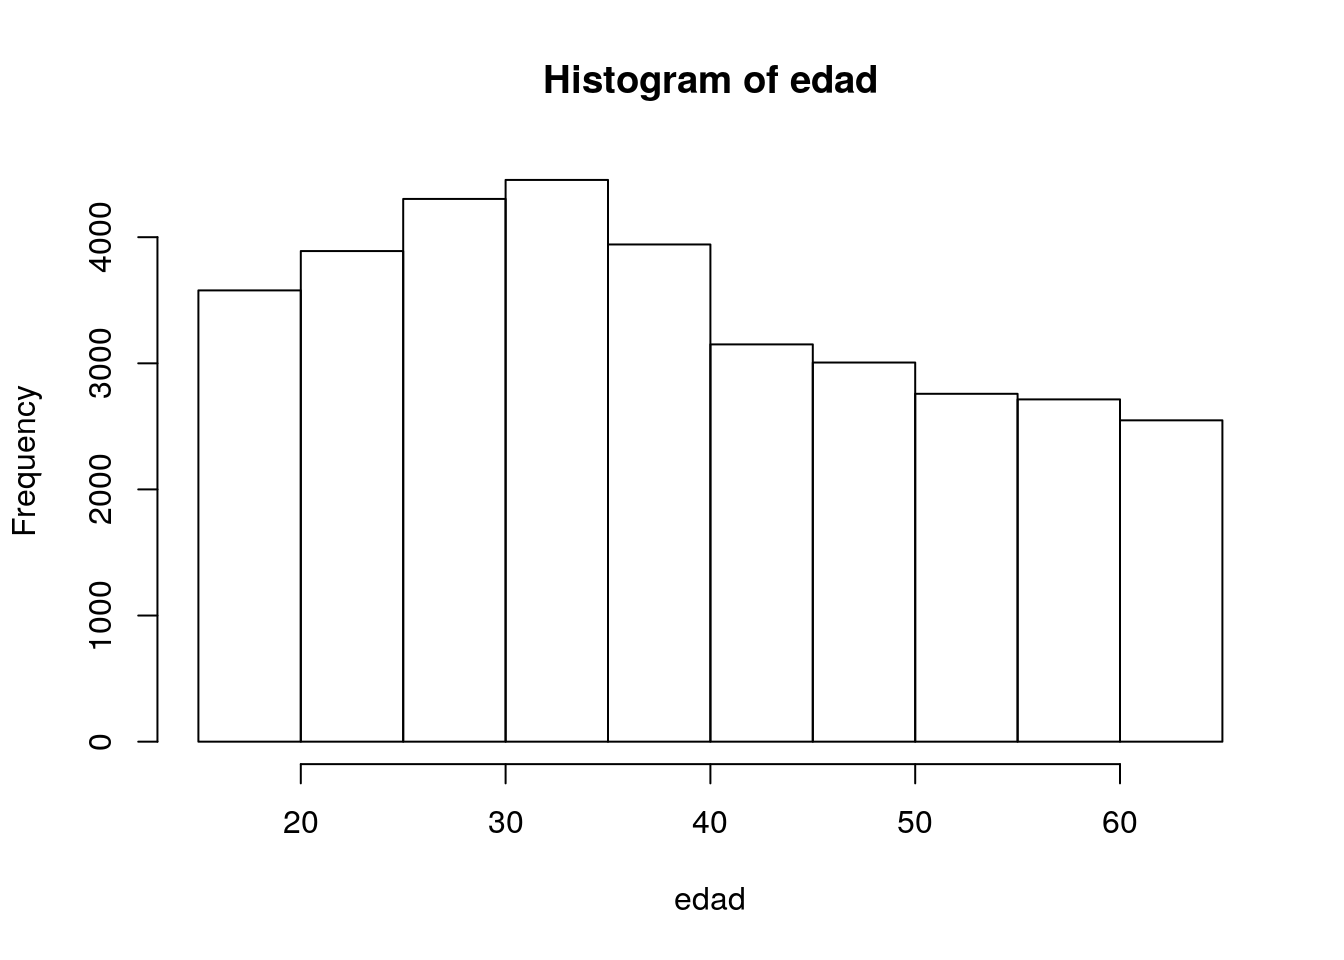
\includegraphics{Introduccion_Datos_files/figure-latex/unnamed-chunk-35-1.pdf}

También podemos representar las frecuencias relativas o los porcentajes.

\begin{Shaded}
\begin{Highlighting}[]
\NormalTok{## Realizamos un histograma con las frecuencias relativas}
\KeywordTok{library}\NormalTok{(lattice)}
\KeywordTok{histogram}\NormalTok{(edad,}
          \DataTypeTok{breaks =} \DecValTok{10}\NormalTok{,}
          \DataTypeTok{ylab =} \StringTok{"Porcentaje del Total"}\NormalTok{)}
\end{Highlighting}
\end{Shaded}

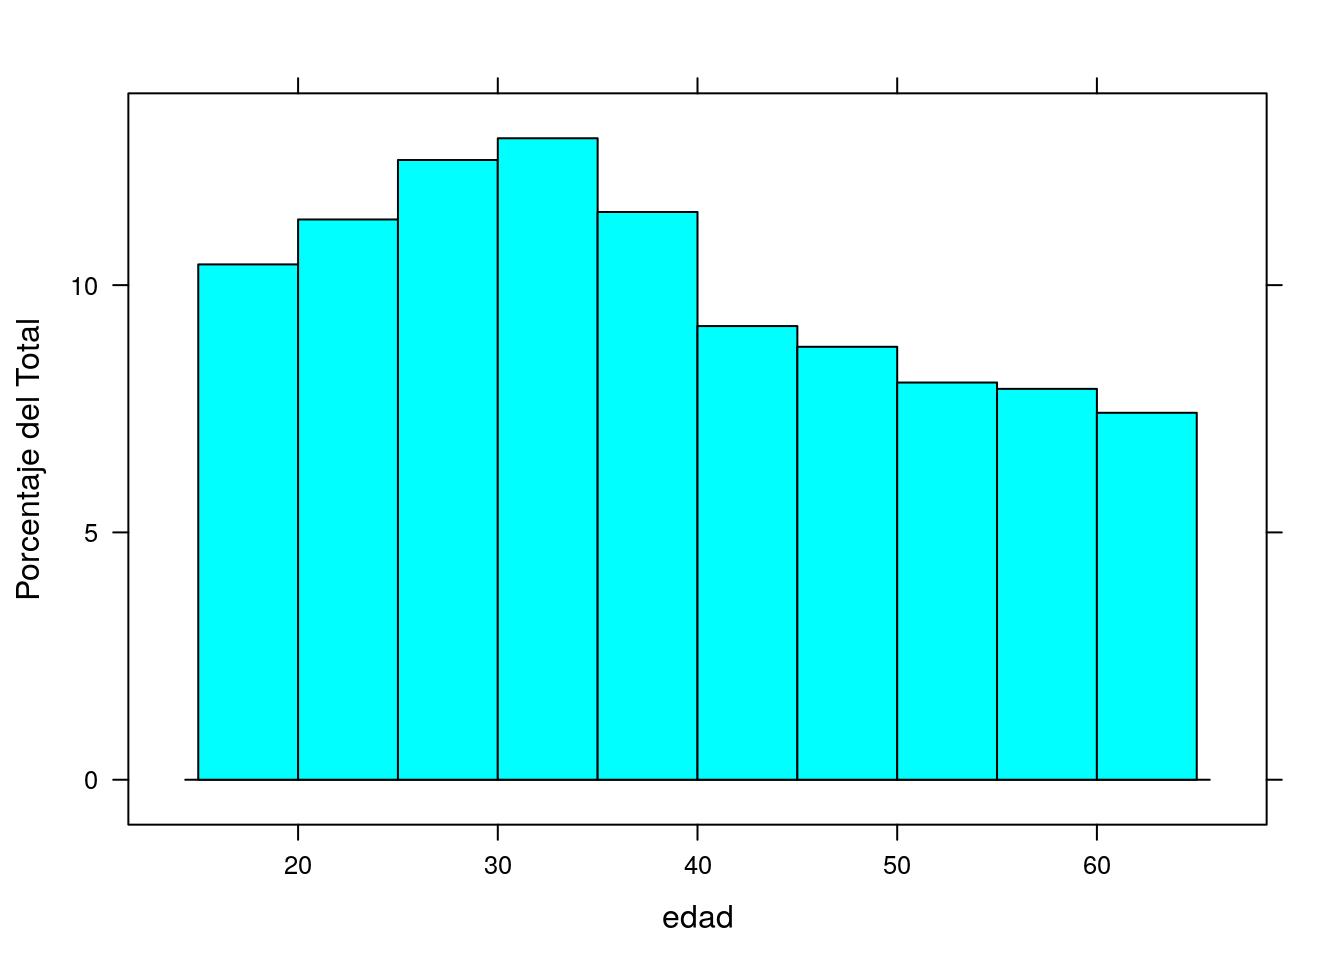
\includegraphics{Introduccion_Datos_files/figure-latex/unnamed-chunk-36-1.pdf}

\begin{Shaded}
\begin{Highlighting}[]
\NormalTok{## Cambiamos el número de barras. Agregamos color}
\KeywordTok{hist}\NormalTok{(}\KeywordTok{as.numeric}\NormalTok{(edad),}
     \DataTypeTok{col =} \StringTok{"seagreen"}\NormalTok{)}
\end{Highlighting}
\end{Shaded}

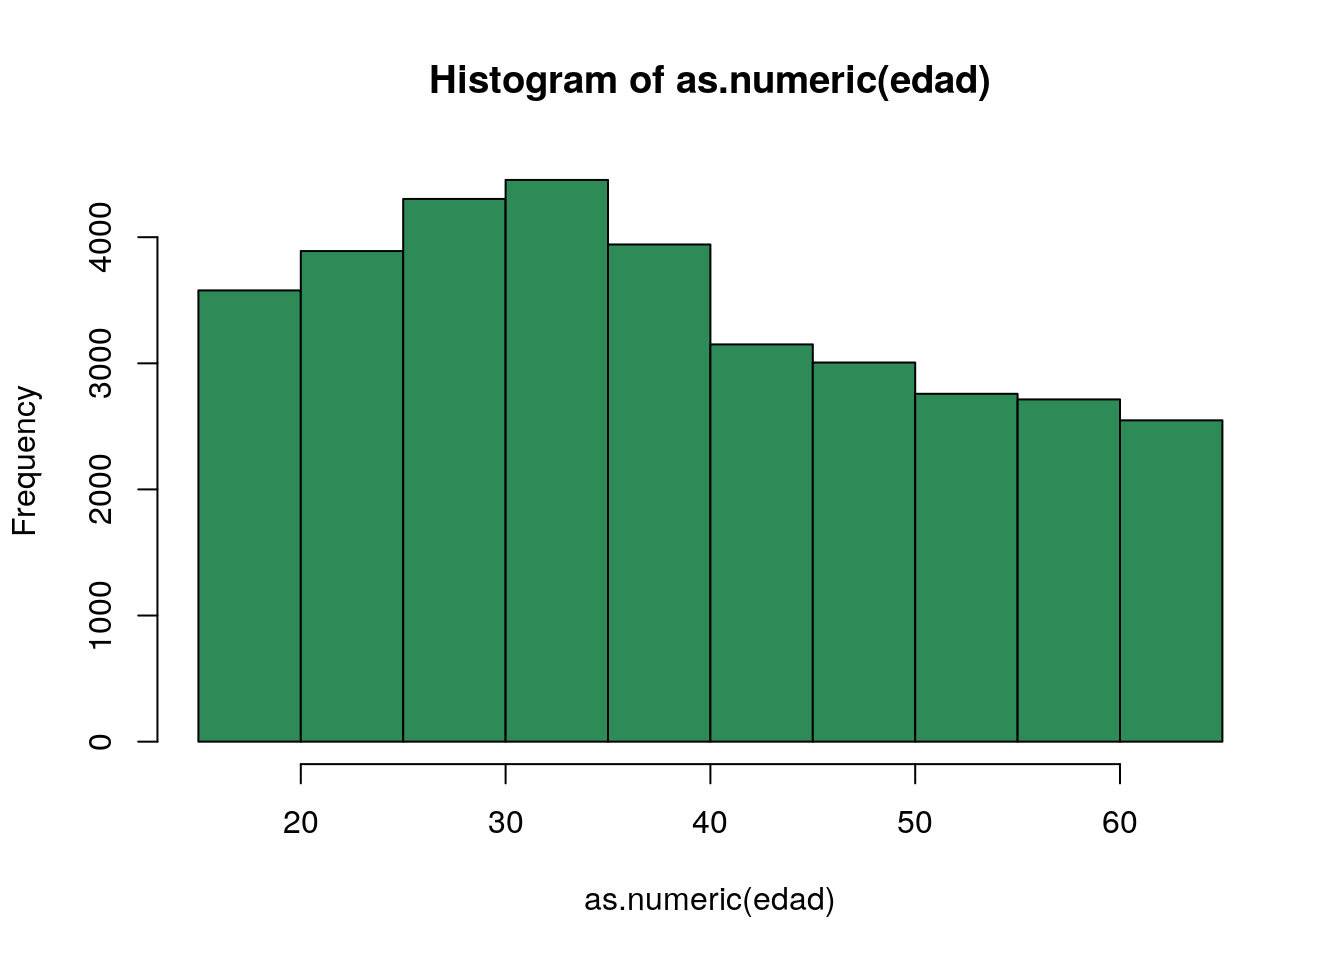
\includegraphics{Introduccion_Datos_files/figure-latex/unnamed-chunk-36-2.pdf}

\begin{Shaded}
\begin{Highlighting}[]
\NormalTok{## Estilamos el gráfico}
\KeywordTok{hist}\NormalTok{(}\KeywordTok{as.numeric}\NormalTok{(edad),}
     \DataTypeTok{axes =} \OtherTok{FALSE}\NormalTok{,}
     \DataTypeTok{main =} \StringTok{"Histograma para edad"}\NormalTok{,}
     \DataTypeTok{xlab =} \StringTok{"Edad"}\NormalTok{,}
     \DataTypeTok{ylab =} \StringTok{"Frecuencia"}\NormalTok{,}
     \CommentTok{# col = "steelblue",}
     \DataTypeTok{xlim =} \KeywordTok{c}\NormalTok{(}\DecValTok{10}\NormalTok{,}\DecValTok{70}\NormalTok{),}
     \DataTypeTok{ylim =} \KeywordTok{c}\NormalTok{(}\DecValTok{0}\NormalTok{, }\DecValTok{5000}\NormalTok{),}
     \DataTypeTok{col =} \KeywordTok{rainbow}\NormalTok{(}\DecValTok{5}\NormalTok{))}
\KeywordTok{axis}\NormalTok{(}\DecValTok{1}\NormalTok{, }\DataTypeTok{pos =} \DecValTok{0}\NormalTok{)}
\KeywordTok{axis}\NormalTok{(}\DecValTok{2}\NormalTok{, }\DataTypeTok{pos =} \DecValTok{10}\NormalTok{)}
\end{Highlighting}
\end{Shaded}

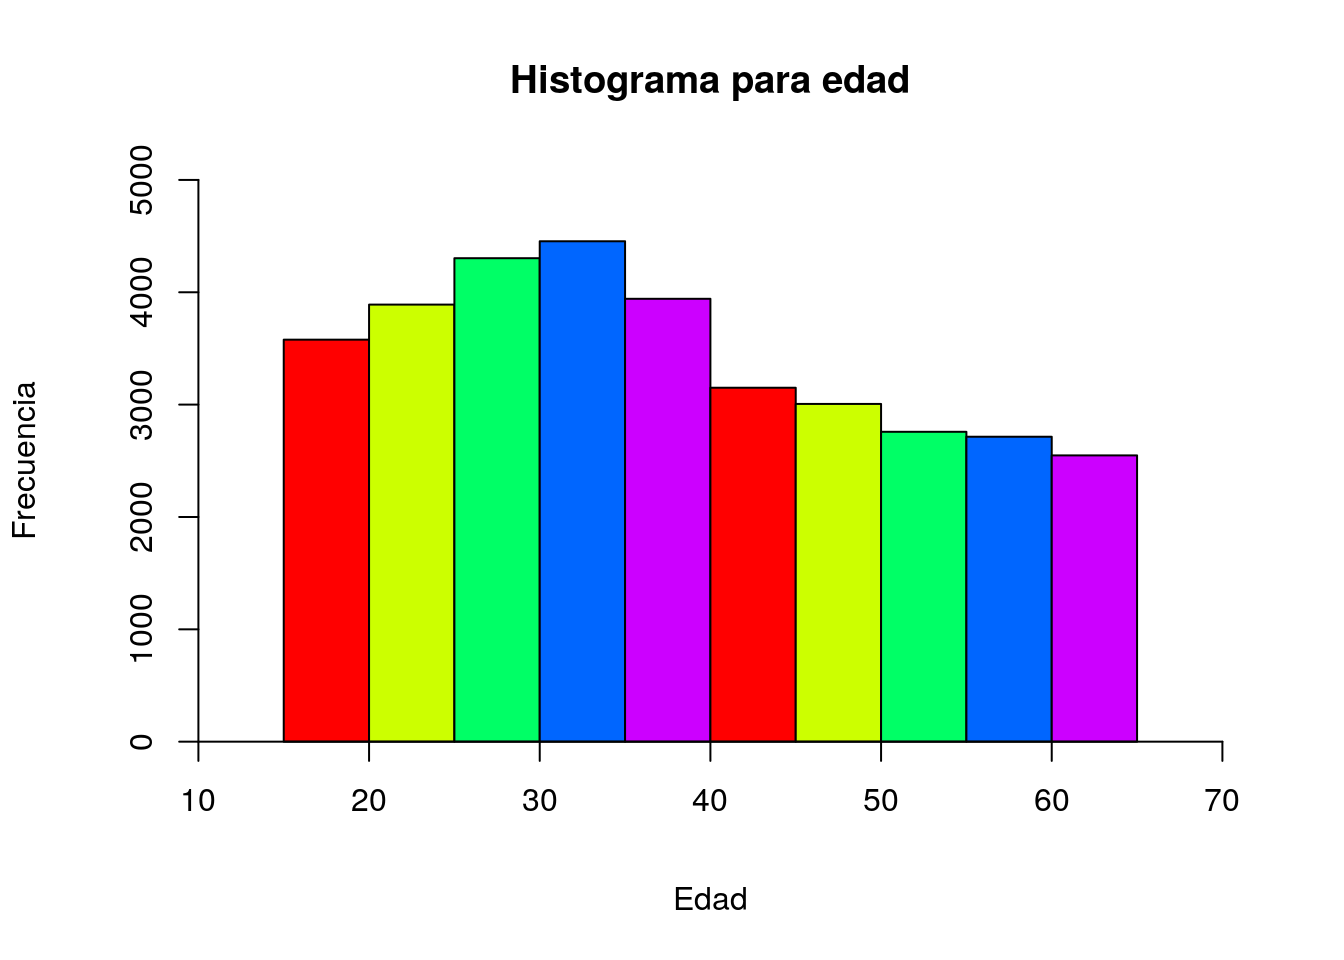
\includegraphics{Introduccion_Datos_files/figure-latex/unnamed-chunk-36-3.pdf}

\section{Gráfico de barras}\label{grafico-de-barras}

El gráfico de barras nos permite visualizar las frecuencias en
\textbf{variables cualitativas}. Para realizar un gráfico de barras
podemo utilizar la función \texttt{barplot}

\begin{Shaded}
\begin{Highlighting}[]
\NormalTok{## Seleccionamos BISG02 y la guardamos en una nueva variable}
\NormalTok{accidente <-}\StringTok{ }\NormalTok{enprecosp}\OperatorTok{$}\NormalTok{BISG02}

\NormalTok{## Convertimos a factor y etiquetamos los códigos de valores}
\NormalTok{accidente <-}\StringTok{ }\KeywordTok{factor}\NormalTok{(accidente,}
                   \DataTypeTok{labels =} \KeywordTok{c}\NormalTok{(}\StringTok{"Sí"}\NormalTok{, }\StringTok{"No"}\NormalTok{, }\StringTok{"Ns/Nc"}\NormalTok{))}
\NormalTok{## Construimos las frecuencias para la variable accidente}
\NormalTok{f <-}\StringTok{ }\KeywordTok{table}\NormalTok{(accidente)}
\NormalTok{frel <-}\StringTok{ }\KeywordTok{prop.table}\NormalTok{(f)}

\NormalTok{## Juntamos todo y armamos una tabla de distribución de freucuencias.}
\NormalTok{dfreq <-}\StringTok{ }\KeywordTok{cbind}\NormalTok{(f, frel)}

\KeywordTok{barplot}\NormalTok{(dfreq[,}\DecValTok{1}\NormalTok{],}
        \DataTypeTok{col =} \StringTok{"steelblue"}\NormalTok{)}
\end{Highlighting}
\end{Shaded}

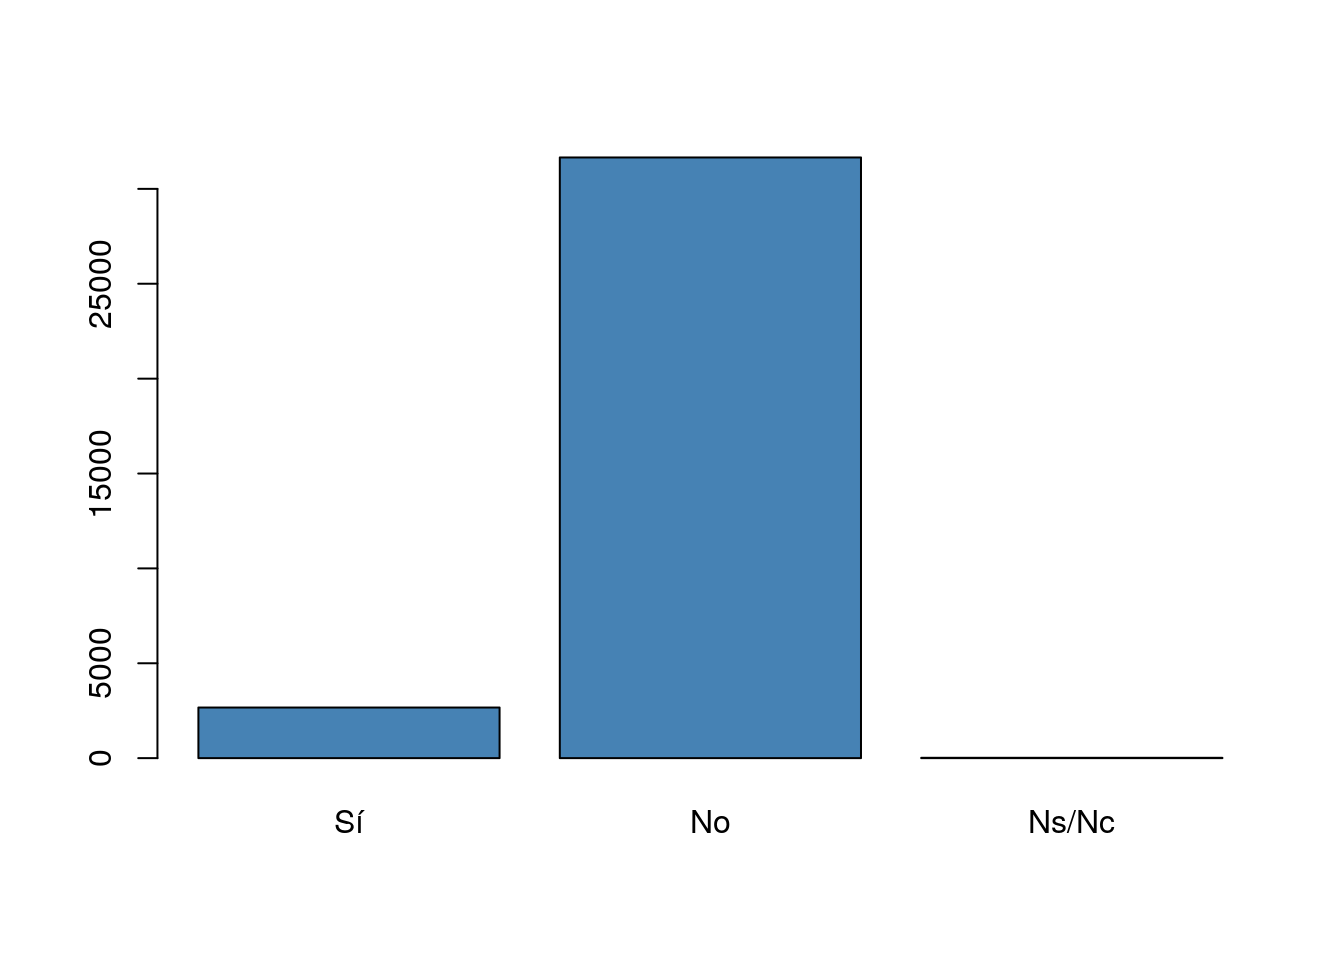
\includegraphics{Introduccion_Datos_files/figure-latex/unnamed-chunk-37-1.pdf}

\section{Gráfico de tortas}\label{grafico-de-tortas}

Los gráficos de tortas también nos permiten graficar frecuencias. Los
gráficos de torta están actualmente desaconsejados. Se aconseja en su
lugar el uso de gráfico de barras. Los gráficos de barras permiten
visualizar más facilemente las diferencias de proporciones que los
gráficos de barras, particularmente cuando representamos más de dos
proporciones. Para ver una revisión acerca de la discusión de gráficos
de barras y de torta vea \citet{spence2005no}. Para realizar un gráfico
de tortas, podemos utilizar la función \texttt{pie}

\begin{Shaded}
\begin{Highlighting}[]
\NormalTok{## Seleccionamos BISG02 y la guardamos en una nueva variable}
\NormalTok{accidente <-}\StringTok{ }\NormalTok{enprecosp}\OperatorTok{$}\NormalTok{BISG02}

\NormalTok{## Convertimos a factor y etiquetamos los códigos de valores}
\NormalTok{accidente <-}\StringTok{ }\KeywordTok{factor}\NormalTok{(accidente,}
                   \DataTypeTok{labels =} \KeywordTok{c}\NormalTok{(}\StringTok{"Sí"}\NormalTok{, }\StringTok{"No"}\NormalTok{, }\StringTok{"Ns/Nc"}\NormalTok{))}
\NormalTok{## Construimos las frecuencias para la variable accidente}
\NormalTok{f <-}\StringTok{ }\KeywordTok{table}\NormalTok{(accidente)}
\NormalTok{frel <-}\StringTok{ }\KeywordTok{prop.table}\NormalTok{(f)}

\KeywordTok{pie}\NormalTok{(frel)}
\end{Highlighting}
\end{Shaded}

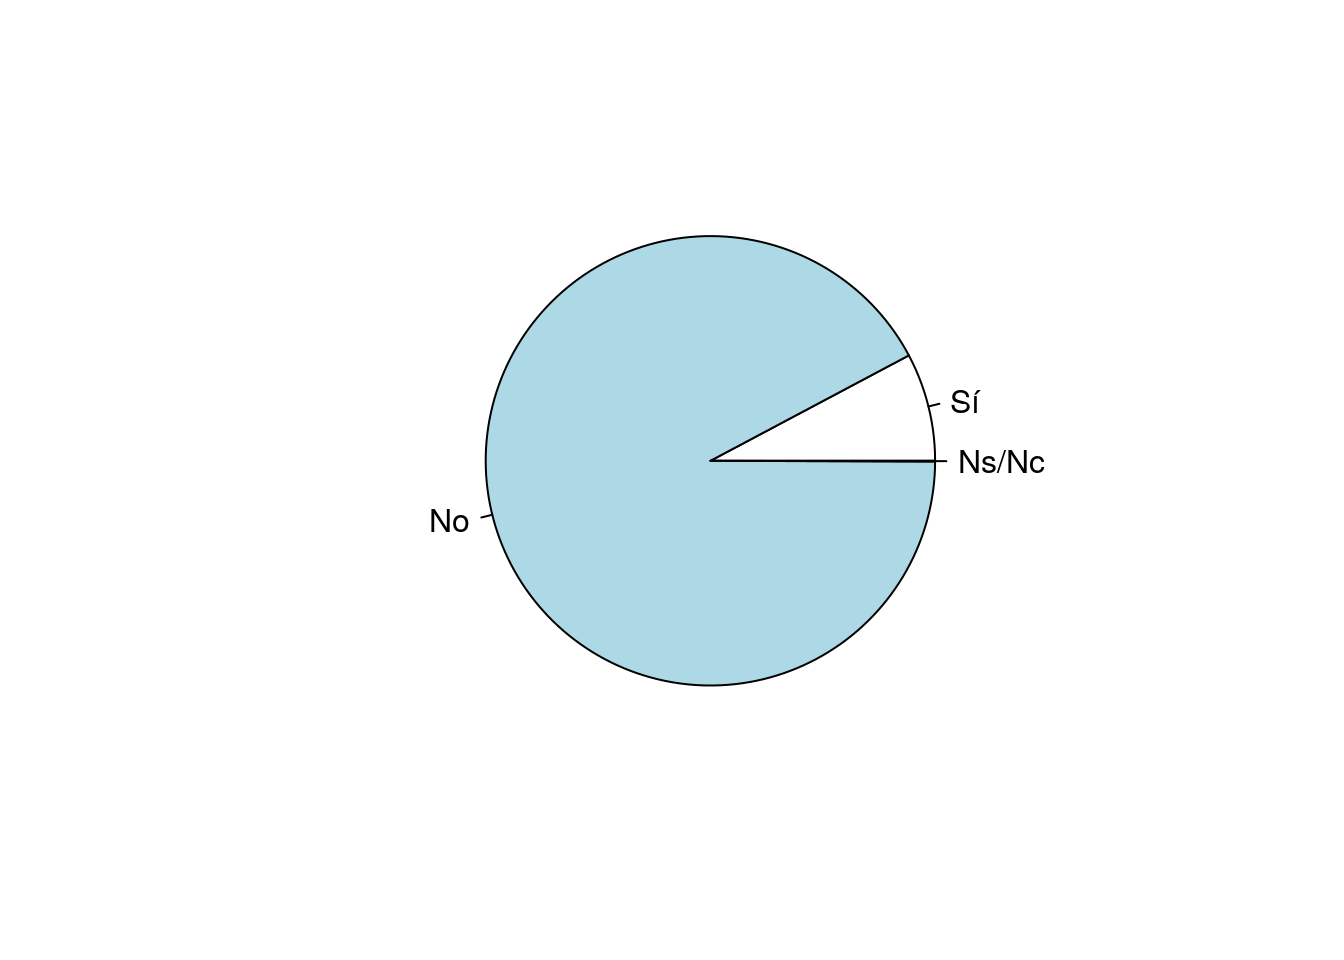
\includegraphics{Introduccion_Datos_files/figure-latex/unnamed-chunk-38-1.pdf}

Estilamos el gráfico. Agregamos los porcentajes.

\begin{Shaded}
\begin{Highlighting}[]
\NormalTok{## Cargamos librería para formatear los porcentajes}
\KeywordTok{library}\NormalTok{(formattable)}

\NormalTok{## Guardamos la tabla con porcentajes en una nueva variables}
\NormalTok{porcentaje <-}\StringTok{ }\KeywordTok{percent}\NormalTok{(frel, }\DataTypeTok{digits =} \DecValTok{2}\NormalTok{, }\DataTypeTok{dec =} \StringTok{","}\NormalTok{)}

\NormalTok{## Construimos las etiquetas}
\NormalTok{etiq <-}\StringTok{ }\KeywordTok{paste}\NormalTok{(}\KeywordTok{names}\NormalTok{(porcentaje),}\StringTok{"; "}\NormalTok{ , }\KeywordTok{round}\NormalTok{(porcentaje, }\DecValTok{4}\NormalTok{), }\DataTypeTok{sep =} \StringTok{""}\NormalTok{)}

\KeywordTok{pie}\NormalTok{(porcentaje,}
    \DataTypeTok{labels =}\NormalTok{ etiq,}
    \DataTypeTok{radius =} \DecValTok{1}\NormalTok{,}
    \DataTypeTok{col =} \KeywordTok{c}\NormalTok{(}\StringTok{"tomato"}\NormalTok{, }\StringTok{"whitesmoke"}\NormalTok{, }\StringTok{"violetred"}\NormalTok{)}
\NormalTok{    )}
\end{Highlighting}
\end{Shaded}

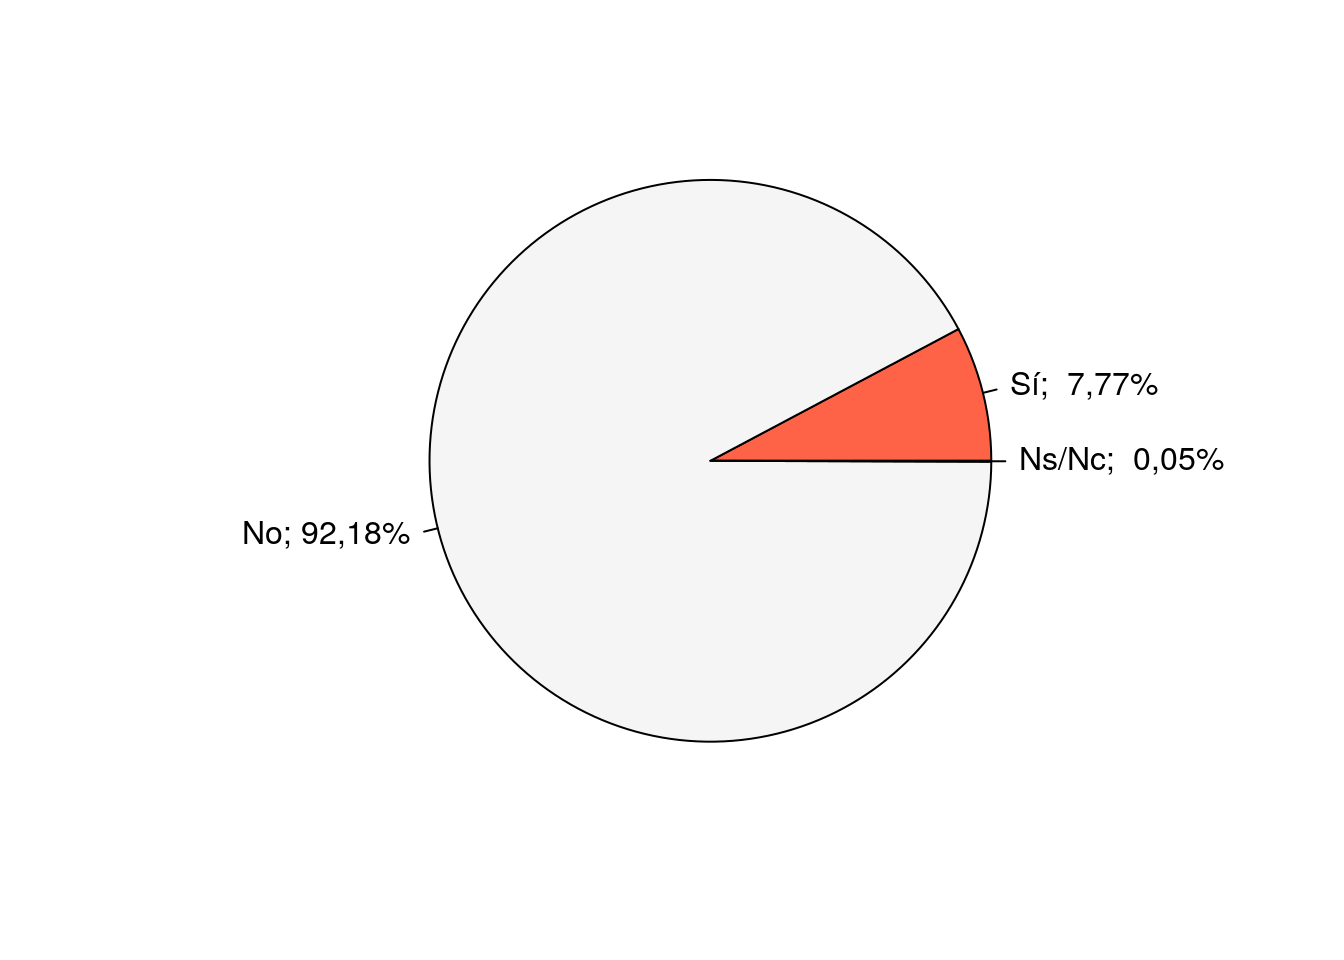
\includegraphics{Introduccion_Datos_files/figure-latex/unnamed-chunk-39-1.pdf}

\section{Ojiva de Galton}\label{ojiva-de-galton}

La ojiva de Galton nos permite graficar las \textbf{frecuencias
relativas acumuladas} y buscar \textbf{percentiles} y \textbf{cuantiles
empíricos}. Veamos como se distribuye la edad de inicio de consumo de
marihuana en la muestra:

\begin{Shaded}
\begin{Highlighting}[]
\NormalTok{## Seleccionamos la edad y la guardamos en una nueva variable}
\NormalTok{## Quito los valores 99, que corresponden a NS/NC}
\NormalTok{edad <-}\StringTok{ }\NormalTok{enprecosp}\OperatorTok{$}\NormalTok{BIMA03[enprecosp}\OperatorTok{$}\NormalTok{BIMA03 }\OperatorTok{!=}\StringTok{ }\DecValTok{99}\NormalTok{]}

\NormalTok{f <-}\StringTok{ }\KeywordTok{table}\NormalTok{(edad)}
\NormalTok{frel <-}\StringTok{ }\KeywordTok{prop.table}\NormalTok{(f)}
\NormalTok{frelcum <-}\StringTok{ }\KeywordTok{cumsum}\NormalTok{(frel)}

\KeywordTok{plot}\NormalTok{(}\KeywordTok{names}\NormalTok{(frelcum), frelcum,}
     \DataTypeTok{type =} \StringTok{"s"}\NormalTok{,}
     \DataTypeTok{ylab =} \StringTok{"F'"}\NormalTok{,}
     \DataTypeTok{xlab =} \StringTok{"Edad"}\NormalTok{)}
\end{Highlighting}
\end{Shaded}

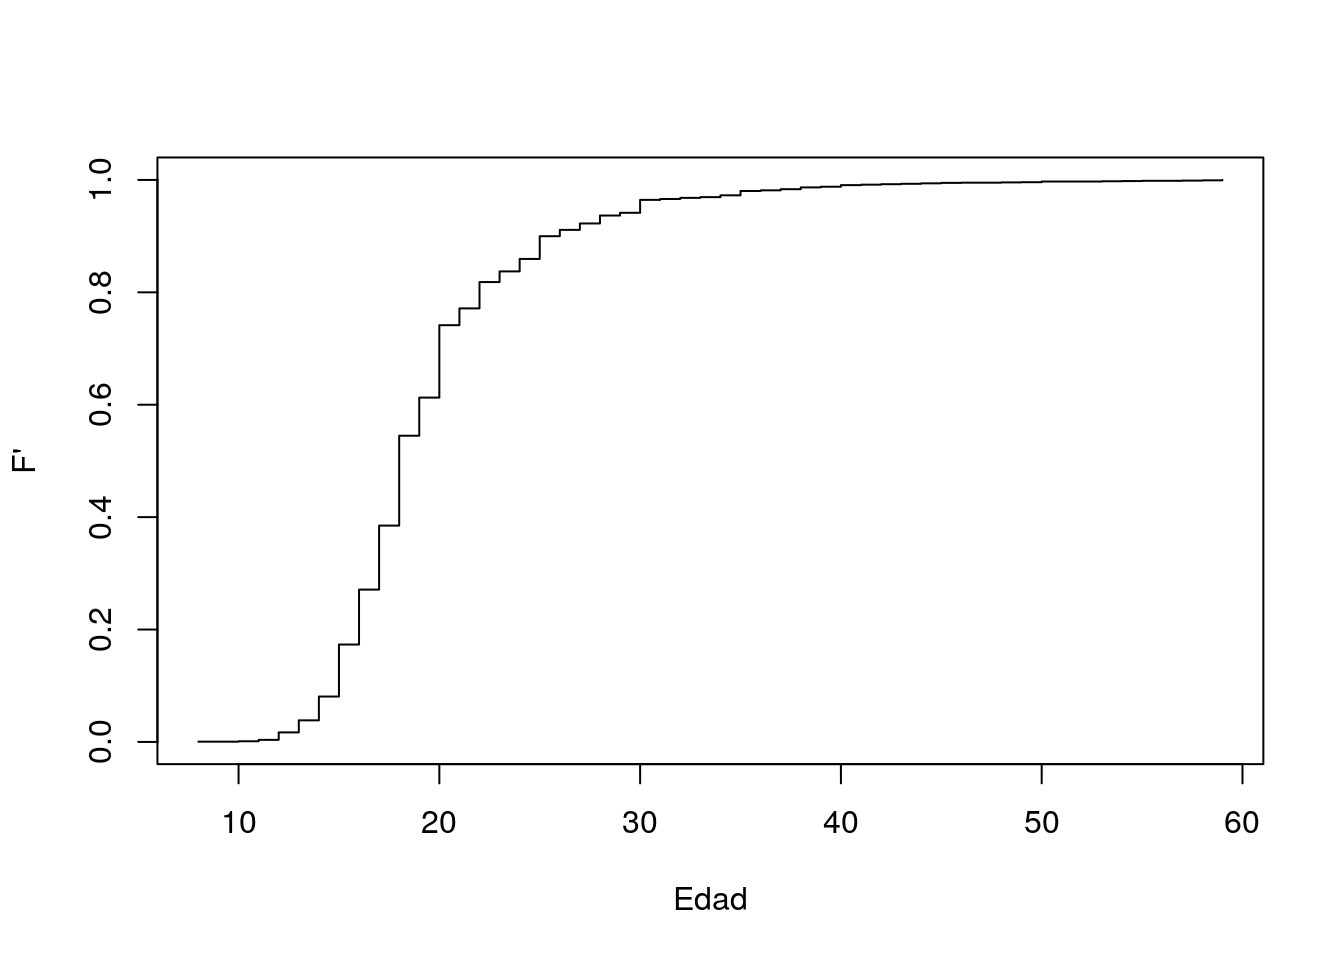
\includegraphics{Introduccion_Datos_files/figure-latex/unnamed-chunk-40-1.pdf}

\begin{Shaded}
\begin{Highlighting}[]
\NormalTok{## Realizamos un gráfico similar, pero utilizando la función}
\NormalTok{## distribución acumulada empírica}
\KeywordTok{plot}\NormalTok{(}\KeywordTok{ecdf}\NormalTok{(edad),}
     \DataTypeTok{main =} \StringTok{"Ojiva de Galton"}\NormalTok{,}
     \DataTypeTok{xlab =} \StringTok{"Edad"}\NormalTok{)}
\end{Highlighting}
\end{Shaded}

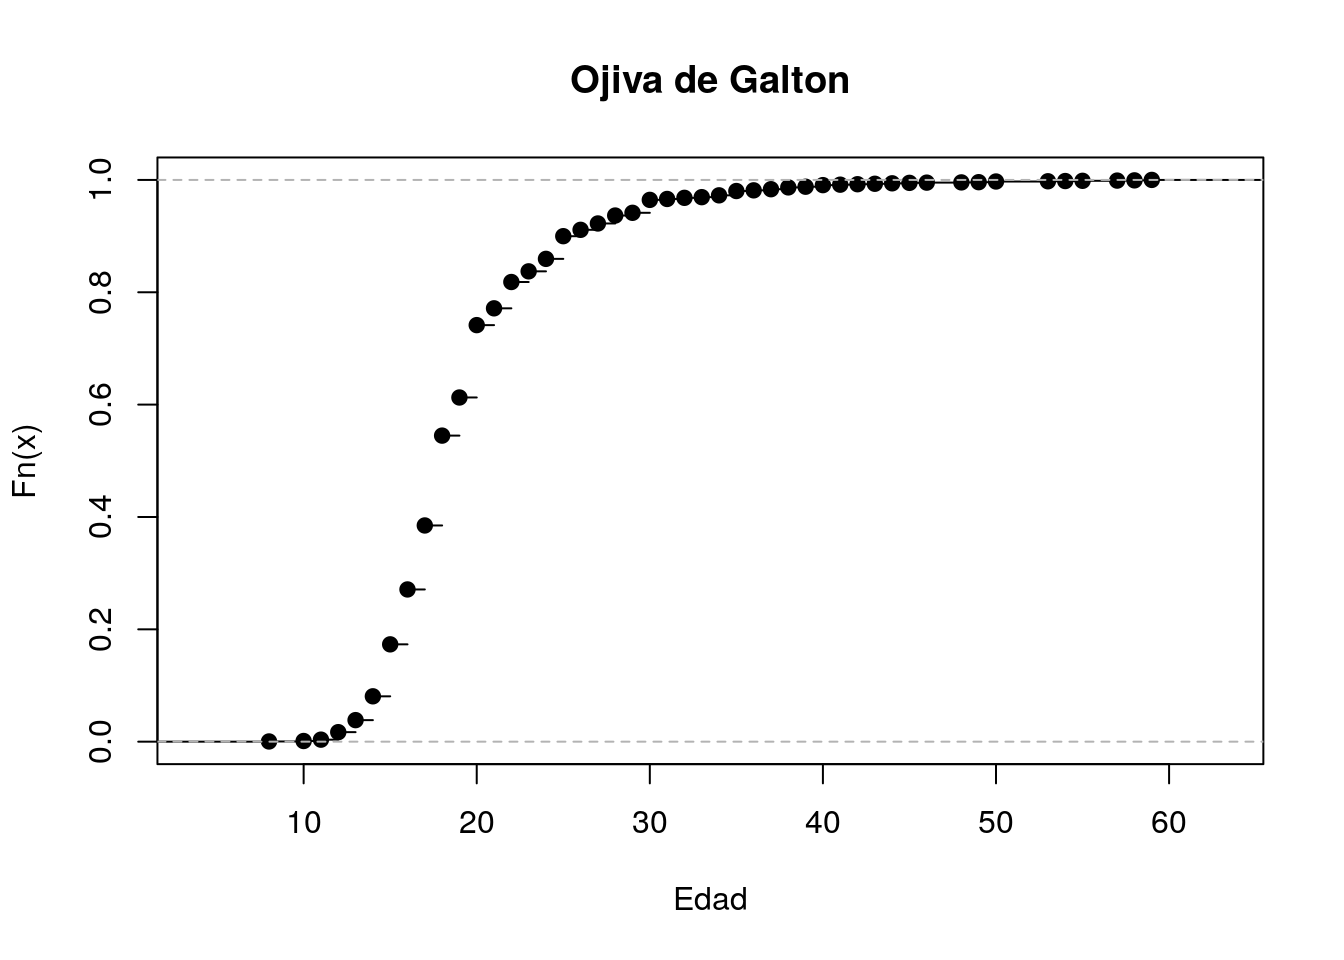
\includegraphics{Introduccion_Datos_files/figure-latex/unnamed-chunk-40-2.pdf}

\chapter{Medidas de resumen}\label{medidas-de-resumen}

\section{Medidas de posición}\label{medidas-de-posicion}

Las medidas de posición nos van a dar información acerca de diferentes
localizaciones de los datos en una variables. Pueden ser
\textbf{centrales}, como la \emph{media}, la \emph{mediana} y la
\emph{moda}. O \textbf{no centrales}, como los \textbf{cuartiles} y
\textbf{percentiles}.

\subsection{Proporción}\label{proporcion}

Es una \textbf{frecuencia relativa}. Vimos varios ejemplos de
proporciones cuando realizamos las tablas de distribución de frecuencia
en el Capítulo \ref{frec}. Calculemos la proporción de personas que
alguna vez en la vida consumieron marihuana.

\begin{Shaded}
\begin{Highlighting}[]
\NormalTok{## Proporción de personas que consumieron marihuana alguna vez en la vida (PV_MA)}
\NormalTok{marihuana <-}\StringTok{ }\NormalTok{enprecosp}\OperatorTok{$}\NormalTok{PV_MA}
\NormalTok{marihuana <-}\StringTok{ }\KeywordTok{factor}\NormalTok{(marihuana,}
                    \DataTypeTok{labels =} \KeywordTok{c}\NormalTok{(}\StringTok{"Sí"}\NormalTok{, }\StringTok{"No"}\NormalTok{)}
\NormalTok{                    )}

\NormalTok{p <-}\StringTok{ }\KeywordTok{prop.table}\NormalTok{(}\KeywordTok{table}\NormalTok{(marihuana))}
\NormalTok{p}
\end{Highlighting}
\end{Shaded}

\begin{verbatim}
## marihuana
##         Sí         No 
## 0.07326093 0.92673907
\end{verbatim}

Entonces, el 7,33\% de los encuestados consumió alguna vez marihuana en
la vida.

\subsection{Moda}\label{moda}

Es el valor de la variable que más se repite. Es el valor de la variable
que tenga la frecuencia más alta.

\begin{Shaded}
\begin{Highlighting}[]
\NormalTok{## En el periodo en que usted consumía marihuana con}
\NormalTok{## mayor frecuencia ¿cada cuánto consumía?}
\NormalTok{fconsumo <-}\StringTok{ }\NormalTok{enprecosp}\OperatorTok{$}\NormalTok{BIMA04}
\NormalTok{fconsumo <-}\StringTok{ }\KeywordTok{factor}\NormalTok{(fconsumo,}
                   \DataTypeTok{levels =} \KeywordTok{c}\NormalTok{(}\DecValTok{1}\OperatorTok{:}\DecValTok{6}\NormalTok{, }\DecValTok{9}\NormalTok{),}
                   \DataTypeTok{labels =} \KeywordTok{c}\NormalTok{(}\StringTok{"Casi todos los días"}\NormalTok{,}
                              \StringTok{"3 0 4 días a la semana"}\NormalTok{,}
                              \StringTok{"1 o 2 días a la semana"}\NormalTok{,}
                              \StringTok{"De 1 a 3 días al mes"}\NormalTok{,}
                              \StringTok{"Menos de una vez al mes"}\NormalTok{,}
                              \StringTok{"Una sola vez"}\NormalTok{,}
                              \StringTok{"Ns/Nc"}\NormalTok{))}

\NormalTok{## Calculamos las frecuencias absolutas}
\NormalTok{p <-}\StringTok{ }\KeywordTok{table}\NormalTok{(fconsumo)}
\NormalTok{p}
\end{Highlighting}
\end{Shaded}

\begin{verbatim}
## fconsumo
##     Casi todos los días  3 0 4 días a la semana  1 o 2 días a la semana 
##                     259                     119                     267 
##    De 1 a 3 días al mes Menos de una vez al mes            Una sola vez 
##                     248                     485                    1120 
##                   Ns/Nc 
##                      18
\end{verbatim}

\begin{Shaded}
\begin{Highlighting}[]
\NormalTok{## Buscamos el valor con la frecuencia máxima}
\KeywordTok{which.max}\NormalTok{(p)}
\end{Highlighting}
\end{Shaded}

\begin{verbatim}
## Una sola vez 
##            6
\end{verbatim}

\subsection{Mediana}\label{mediana}

Es el valor de la variable que deja por debajo y por arriba, el 50\% de
los casos. Podemos calcularla a partir de variables de \textbf{nivel
ordinal}. La podemos observar a partir de las frecuencias relativas
acumuladas. Continuando con la frecuencia de consumo de marihuana

\begin{Shaded}
\begin{Highlighting}[]
\NormalTok{## En el periodo en que usted consumía marihuana con}
\NormalTok{## mayor frecuencia ¿cada cuánto consumía?}
\NormalTok{fconsumo <-}\StringTok{ }\NormalTok{enprecosp}\OperatorTok{$}\NormalTok{BIMA04}

\NormalTok{## Excluimos el valor 9, Ns/Nc}
\NormalTok{fconsumo <-}\StringTok{ }\KeywordTok{factor}\NormalTok{(fconsumo,}
                   \DataTypeTok{levels =} \KeywordTok{c}\NormalTok{(}\DecValTok{6}\OperatorTok{:}\DecValTok{1}\NormalTok{),}
                   \DataTypeTok{labels =} \KeywordTok{c}\NormalTok{(}\StringTok{"Una sola vez"}\NormalTok{,}
                              \StringTok{"Menos de una vez al mes"}\NormalTok{,}
                              \StringTok{"De 1 a 3 días al mes"}\NormalTok{,}
                              \StringTok{"1 o 2 días a la semana"}\NormalTok{,}
                              \StringTok{"3 o 4 días a la semana"}\NormalTok{,}
                              \StringTok{"Casi todos los días"}
\NormalTok{                              ),}
                   \DataTypeTok{ordered =} \OtherTok{TRUE}\NormalTok{)}

\NormalTok{## Frecuencias absolutas}
\NormalTok{frec <-}\StringTok{ }\KeywordTok{table}\NormalTok{(fconsumo)}
\NormalTok{## Frecuencias relativas}
\NormalTok{frel <-}\StringTok{ }\KeywordTok{prop.table}\NormalTok{(frec)}
\NormalTok{## Frecuencias relativas acumuladas}
\NormalTok{cumfrel <-}\StringTok{ }\KeywordTok{cumsum}\NormalTok{(frel)}
\NormalTok{cumfrel}
\end{Highlighting}
\end{Shaded}

\begin{verbatim}
##            Una sola vez Menos de una vez al mes    De 1 a 3 días al mes 
##               0.4483587               0.6425140               0.7417934 
##  1 o 2 días a la semana  3 o 4 días a la semana     Casi todos los días 
##               0.8486789               0.8963171               1.0000000
\end{verbatim}

El primer valor que supera 0.5 es la mediana. En este caso, la mediana
es \emph{menos de una vez al mes}.

\subsection{Cuartiles y percentiles}\label{cuartiles-y-percentiles}

Los cuartiles dividen al conjunto de datos en 4. El primer cuartil
(\textbf{1Q}) es el valor de la variable que deja por debajo el 25\% de
los casos. El tercer cuartil (\textbf{3er cuartil}) es el valor de la
variable que deja por debajo el 75\% de los casos. El segundo cuartil
(\textbf{2Q}) es el valor que deja por debajo el 25\% de los casos. Es
la \textbf{mediana}.\\
Si dividimos a la distribución de datos en 100, obtenemos los
\textbf{percentiles}. El \textbf{percentil r} es el valor de la variable
que deja el r por ciento de los casos por debajo de él. Utilicemos estas
medidas para comparar la edad de inicio de consumo de alcohol, tabaco y
marihuana.

\begin{Shaded}
\begin{Highlighting}[]
\NormalTok{## Seleccionamos las variables de edad de inicio de consumo}
\NormalTok{## para tabaco, alcohol y marihuana}
\NormalTok{edad_tabaco <-}\StringTok{ }\NormalTok{enprecosp}\OperatorTok{$}\NormalTok{BITA03[enprecosp}\OperatorTok{$}\NormalTok{BITA03 }\OperatorTok{!=}\StringTok{ }\DecValTok{99}\NormalTok{]}
\NormalTok{edad_alcohol <-}\StringTok{ }\NormalTok{enprecosp}\OperatorTok{$}\NormalTok{BIBA03[enprecosp}\OperatorTok{$}\NormalTok{BIBA03 }\OperatorTok{!=}\StringTok{ }\DecValTok{99}\NormalTok{]}
\NormalTok{edad_marihuana <-}\StringTok{ }\NormalTok{enprecosp}\OperatorTok{$}\NormalTok{BIMA03[enprecosp}\OperatorTok{$}\NormalTok{BIMA03 }\OperatorTok{!=}\StringTok{ }\DecValTok{99}\NormalTok{]}

\NormalTok{## Calculamos los cuantiles}
\KeywordTok{quantile}\NormalTok{(edad_tabaco, }\DataTypeTok{na.rm =} \OtherTok{TRUE}\NormalTok{)}
\end{Highlighting}
\end{Shaded}

\begin{verbatim}
##   0%  25%  50%  75% 100% 
##    3   15   16   18   64
\end{verbatim}

\begin{Shaded}
\begin{Highlighting}[]
\KeywordTok{quantile}\NormalTok{(edad_alcohol, }\DataTypeTok{na.rm =} \OtherTok{TRUE}\NormalTok{)}
\end{Highlighting}
\end{Shaded}

\begin{verbatim}
##   0%  25%  50%  75% 100% 
##    1   15   17   20   64
\end{verbatim}

\begin{Shaded}
\begin{Highlighting}[]
\KeywordTok{quantile}\NormalTok{(edad_marihuana, }\DataTypeTok{na.rm =} \OtherTok{TRUE}\NormalTok{)}
\end{Highlighting}
\end{Shaded}

\begin{verbatim}
##   0%  25%  50%  75% 100% 
##    8   16   18   21   59
\end{verbatim}

\begin{Shaded}
\begin{Highlighting}[]
\NormalTok{## Calculamos los percentiles 5 y 95}
\KeywordTok{quantile}\NormalTok{(edad_tabaco, }\KeywordTok{c}\NormalTok{(}\FloatTok{0.05}\NormalTok{, }\FloatTok{0.95}\NormalTok{), }\DataTypeTok{na.rm =} \OtherTok{TRUE}\NormalTok{)}
\end{Highlighting}
\end{Shaded}

\begin{verbatim}
##  5% 95% 
##  12  25
\end{verbatim}

\begin{Shaded}
\begin{Highlighting}[]
\KeywordTok{quantile}\NormalTok{(edad_alcohol, }\KeywordTok{c}\NormalTok{(}\FloatTok{0.05}\NormalTok{, }\FloatTok{0.95}\NormalTok{), }\DataTypeTok{na.rm =} \OtherTok{TRUE}\NormalTok{)}
\end{Highlighting}
\end{Shaded}

\begin{verbatim}
##  5% 95% 
##  13  26
\end{verbatim}

\begin{Shaded}
\begin{Highlighting}[]
\KeywordTok{quantile}\NormalTok{(edad_marihuana, }\KeywordTok{c}\NormalTok{(}\FloatTok{0.05}\NormalTok{, }\FloatTok{0.95}\NormalTok{), }\DataTypeTok{na.rm =} \OtherTok{TRUE}\NormalTok{)}
\end{Highlighting}
\end{Shaded}

\begin{verbatim}
##  5% 95% 
##  14  30
\end{verbatim}

\subsection{Media}\label{media}

Es el promedio. Se obtiene sumando todos los datos y dividiendo por el
número de casos.

\[
\bar{x} = \frac{\displaystyle \sum_{i=1}^n x_i}{n}
\] La media, a diferencia de la mediana, es sensible a valores extremos.
Observemos un ejemplo.

\begin{Shaded}
\begin{Highlighting}[]
\NormalTok{## Cantidad de miembros en el hogar}
\NormalTok{nhogar <-}\StringTok{ }\NormalTok{enprecosp}\OperatorTok{$}\NormalTok{CNTDDCOMP}
\KeywordTok{range}\NormalTok{(nhogar)}
\end{Highlighting}
\end{Shaded}

\begin{verbatim}
## [1]  1 24
\end{verbatim}

\begin{Shaded}
\begin{Highlighting}[]
\NormalTok{## Graficamos}
\KeywordTok{hist}\NormalTok{(nhogar)}
\end{Highlighting}
\end{Shaded}

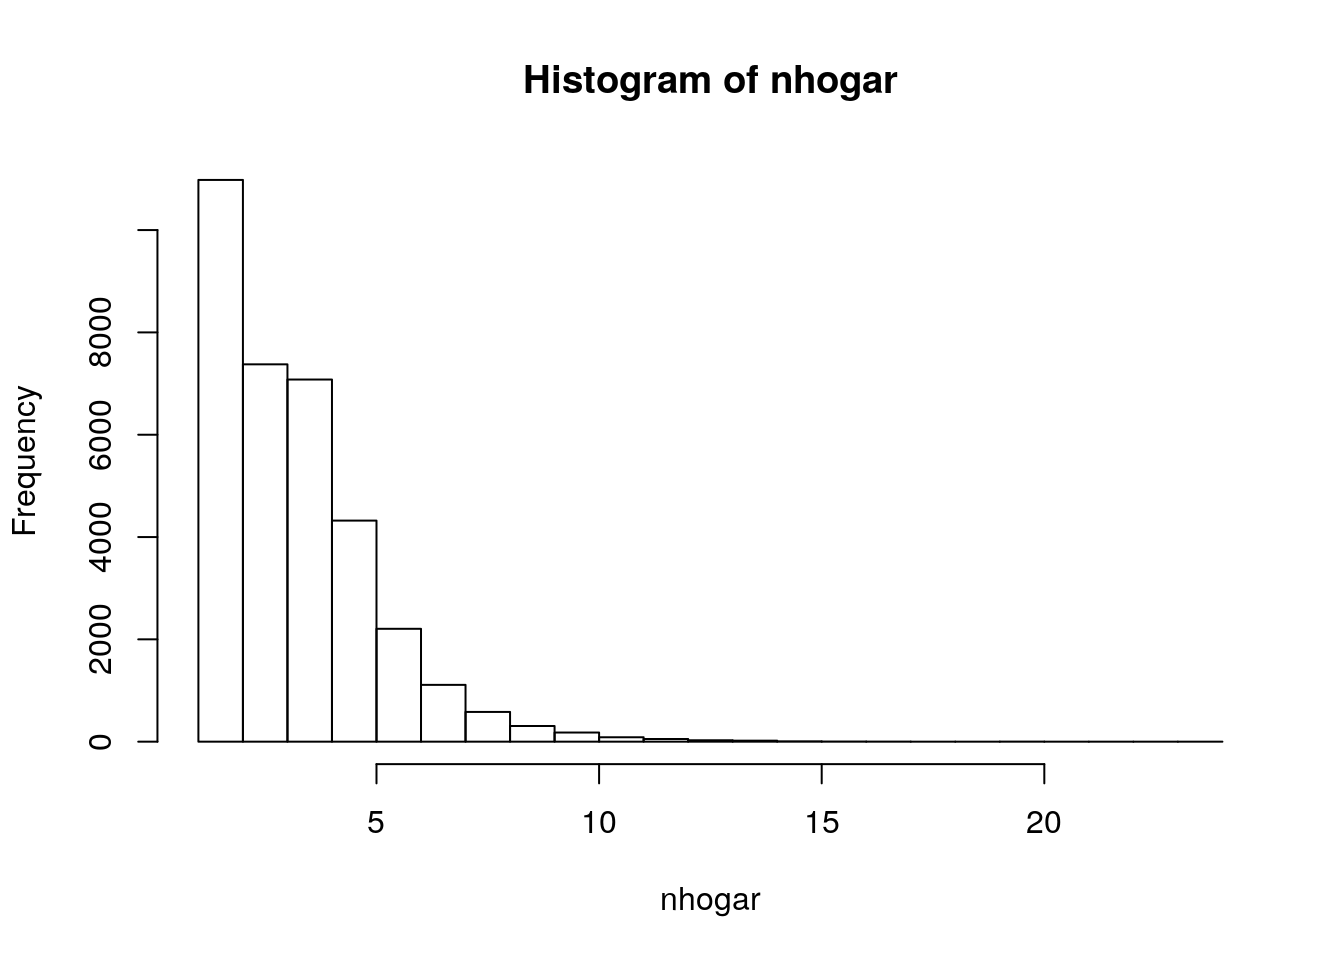
\includegraphics{Introduccion_Datos_files/figure-latex/unnamed-chunk-46-1.pdf}

\begin{Shaded}
\begin{Highlighting}[]
\NormalTok{## Calculamos las medidas de resumen}
\KeywordTok{sum}\NormalTok{(nhogar)}\OperatorTok{/}\KeywordTok{length}\NormalTok{(nhogar)}
\end{Highlighting}
\end{Shaded}

\begin{verbatim}
## [1] 3.572751
\end{verbatim}

\begin{Shaded}
\begin{Highlighting}[]
\KeywordTok{mean}\NormalTok{(nhogar)}
\end{Highlighting}
\end{Shaded}

\begin{verbatim}
## [1] 3.572751
\end{verbatim}

\begin{Shaded}
\begin{Highlighting}[]
\KeywordTok{median}\NormalTok{(nhogar)}
\end{Highlighting}
\end{Shaded}

\begin{verbatim}
## [1] 3
\end{verbatim}

\section{Medidas de dispersión}\label{medidas-de-dispersion}

Son medidas que nos indican el grado de agrupación de los datos

\subsection{Rango o recorrido}\label{rango-o-recorrido}

Es la distancia entre el valor máximo y el valor mínimo.

\[
R = x_{n} - x_{1}
\] Donde:\\
\(x_n\) es el valor máximo\\
\(x_1\) es el valor mínimo

\begin{Shaded}
\begin{Highlighting}[]
\NormalTok{## Veamos cual es el rango de la variables cantidad de miembros del hogar}
\NormalTok{nhogar <-}\StringTok{ }\NormalTok{enprecosp}\OperatorTok{$}\NormalTok{CNTDDCOMP}
\KeywordTok{range}\NormalTok{(nhogar)}
\end{Highlighting}
\end{Shaded}

\begin{verbatim}
## [1]  1 24
\end{verbatim}

\begin{Shaded}
\begin{Highlighting}[]
\NormalTok{## Rango para cantidad de habitaciones del hogar}
\NormalTok{nhabitaciones <-}\StringTok{ }\NormalTok{enprecosp}\OperatorTok{$}\NormalTok{BHHO02}
\KeywordTok{range}\NormalTok{(nhabitaciones)}
\end{Highlighting}
\end{Shaded}

\begin{verbatim}
## [1]  0 20
\end{verbatim}

También son de utilidad el \textbf{rango o recorrido intercuartilar} y
el \textbf{rango o recorrido semi-intercuartilar}.\\
El \textbf{rango o recorrido intercuartilar} se simboliza con AIQ y es
la distancia entre el tercer y el primer cuartil. El \textbf{rango o
recorrido intercuartilar} se simboliza con SRIC y es la mitad del AIQ.
Calulemos estas distancias para el tiempo de consumo de tabaco, alcohol
y marihuana.

\begin{Shaded}
\begin{Highlighting}[]
\NormalTok{## Seleccionamos las variables de edad de inicio de consumo}
\NormalTok{## para tabaco, alcohol y marihuana}
\NormalTok{edad_tabaco <-}\StringTok{ }\NormalTok{enprecosp}\OperatorTok{$}\NormalTok{BITA03[enprecosp}\OperatorTok{$}\NormalTok{BITA03 }\OperatorTok{!=}\StringTok{ }\DecValTok{99}\NormalTok{]}
\NormalTok{edad_alcohol <-}\StringTok{ }\NormalTok{enprecosp}\OperatorTok{$}\NormalTok{BIBA03[enprecosp}\OperatorTok{$}\NormalTok{BIBA03 }\OperatorTok{!=}\StringTok{ }\DecValTok{99}\NormalTok{]}
\NormalTok{edad_marihuana <-}\StringTok{ }\NormalTok{enprecosp}\OperatorTok{$}\NormalTok{BIMA03[enprecosp}\OperatorTok{$}\NormalTok{BIMA03 }\OperatorTok{!=}\StringTok{ }\DecValTok{99}\NormalTok{]}

\NormalTok{## Calculamos los cuantiles}
\NormalTok{q_tabaco <-}\StringTok{ }\KeywordTok{quantile}\NormalTok{(edad_tabaco, }\DataTypeTok{na.rm =} \OtherTok{TRUE}\NormalTok{)}
\NormalTok{q_alcohol <-}\StringTok{ }\KeywordTok{quantile}\NormalTok{(edad_alcohol, }\DataTypeTok{na.rm =} \OtherTok{TRUE}\NormalTok{)}
\NormalTok{q_marihuana <-}\StringTok{ }\KeywordTok{quantile}\NormalTok{(edad_marihuana, }\DataTypeTok{na.rm =} \OtherTok{TRUE}\NormalTok{)}

\NormalTok{## Calculamos el rango intercuartilar}
\NormalTok{aiq_t <-}\StringTok{ }\NormalTok{q_tabaco[}\DecValTok{4}\NormalTok{] }\OperatorTok{-}\StringTok{ }\NormalTok{q_tabaco[}\DecValTok{2}\NormalTok{]; aiq_t}
\end{Highlighting}
\end{Shaded}

\begin{verbatim}
## 75% 
##   3
\end{verbatim}

\begin{Shaded}
\begin{Highlighting}[]
\NormalTok{aiq_al <-}\StringTok{ }\NormalTok{q_alcohol[}\DecValTok{4}\NormalTok{] }\OperatorTok{-}\StringTok{ }\NormalTok{q_alcohol[}\DecValTok{2}\NormalTok{]; aiq_al}
\end{Highlighting}
\end{Shaded}

\begin{verbatim}
## 75% 
##   5
\end{verbatim}

\begin{Shaded}
\begin{Highlighting}[]
\NormalTok{aiq_ma <-}\StringTok{ }\NormalTok{q_marihuana[}\DecValTok{4}\NormalTok{] }\OperatorTok{-}\StringTok{ }\NormalTok{q_marihuana[}\DecValTok{2}\NormalTok{]; aiq_ma}
\end{Highlighting}
\end{Shaded}

\begin{verbatim}
## 75% 
##   5
\end{verbatim}

\begin{Shaded}
\begin{Highlighting}[]
\NormalTok{## Calculamos el rango semi-itercuartilar}
\NormalTok{aiq_t}\OperatorTok{/}\DecValTok{2}
\end{Highlighting}
\end{Shaded}

\begin{verbatim}
## 75% 
## 1.5
\end{verbatim}

\begin{Shaded}
\begin{Highlighting}[]
\NormalTok{aiq_al}\OperatorTok{/}\DecValTok{2}
\end{Highlighting}
\end{Shaded}

\begin{verbatim}
## 75% 
## 2.5
\end{verbatim}

\begin{Shaded}
\begin{Highlighting}[]
\NormalTok{aiq_ma}\OperatorTok{/}\DecValTok{2}
\end{Highlighting}
\end{Shaded}

\begin{verbatim}
## 75% 
## 2.5
\end{verbatim}

\subsection{Varianza y desvío
estándar}\label{varianza-y-desvio-estandar}

Una de las medidas más utilizadas para medir la variabilidad cuando los
datos son cuantitativos es la varianza (\(s^2\)) y el desvío estándar
(\(s\)).

Sea n la cantidad de casos. La \textbf{varianza} es la suma de los
cuadrados de los desvíos con respecto a la media, dividido por n - 1.

\[
s^2 = \frac{\sum_{i=1}^n (x_i - \bar{x})^2}{n - 1}
\] El \textbf{desvío estándar} es la raíz cuadrada de la varianza.

\[
s = \sqrt{s^2}
\]

\begin{Shaded}
\begin{Highlighting}[]
\NormalTok{## Calculemos la varianza para los edad de}
\NormalTok{## Inicio de consumo de tabaco}
\NormalTok{## Quitamos los valores faltantes}
\NormalTok{edad_tabaco <-}\StringTok{ }\NormalTok{edad_tabaco[}\OperatorTok{!}\KeywordTok{is.na}\NormalTok{(edad_tabaco)]}

\NormalTok{## Calculo la varianza}
\NormalTok{n <-}\StringTok{ }\KeywordTok{length}\NormalTok{(edad_tabaco)}
\NormalTok{xn <-}\StringTok{ }\KeywordTok{mean}\NormalTok{(edad_tabaco)}
\NormalTok{s2 <-}\StringTok{ }\KeywordTok{sum}\NormalTok{((edad_tabaco }\OperatorTok{-}\StringTok{ }\NormalTok{xn)}\OperatorTok{^}\DecValTok{2}\NormalTok{) }\OperatorTok{/}\StringTok{ }\NormalTok{(n }\OperatorTok{-}\StringTok{ }\DecValTok{1}\NormalTok{); s2}
\end{Highlighting}
\end{Shaded}

\begin{verbatim}
## [1] 19.81292
\end{verbatim}

\begin{Shaded}
\begin{Highlighting}[]
\NormalTok{## Desvío estándar}
\KeywordTok{sqrt}\NormalTok{(s2)}
\end{Highlighting}
\end{Shaded}

\begin{verbatim}
## [1] 4.45117
\end{verbatim}

\begin{Shaded}
\begin{Highlighting}[]
\NormalTok{## Utilizando la función sd}
\KeywordTok{var}\NormalTok{(edad_tabaco)}
\end{Highlighting}
\end{Shaded}

\begin{verbatim}
## [1] 19.81292
\end{verbatim}

\begin{Shaded}
\begin{Highlighting}[]
\KeywordTok{sd}\NormalTok{(edad_tabaco)}
\end{Highlighting}
\end{Shaded}

\begin{verbatim}
## [1] 4.45117
\end{verbatim}

\begin{Shaded}
\begin{Highlighting}[]
\NormalTok{## Calculamos sd para alcohol y marihuana}
\KeywordTok{sd}\NormalTok{(edad_alcohol, }\DataTypeTok{na.rm =} \OtherTok{TRUE}\NormalTok{)}
\end{Highlighting}
\end{Shaded}

\begin{verbatim}
## [1] 4.705321
\end{verbatim}

\begin{Shaded}
\begin{Highlighting}[]
\KeywordTok{sd}\NormalTok{(edad_marihuana, }\DataTypeTok{na.rm =} \OtherTok{TRUE}\NormalTok{)}
\end{Highlighting}
\end{Shaded}

\begin{verbatim}
## [1] 5.476129
\end{verbatim}

La varianza y el desvío estandar dependen de la unidad de medida que se
utilice. Por ejemplo, la varianza de la edad de inicio de consumo de
alcohol se mide en años al cuadrado. Y el desvío en años. Ello hace que
la medida sea diferente si utilizamos escalas diferentes. Imaginemos que
medimos el peso de un grupo de personas en gramos y en kilos. La
varianza, para ese grupo de personas, medida en \(gramos^2\) será más
grande que cuando la midamos en \(kilos^2\).\\
A veces, incluso, nos interesa comparar magnitudes diferentes, por
ejemplo, peso y altura, y comparar la varianza de ambas variables. Para
poder interpretar más facilmente el desvío estandar en términos
relativos se utiliza el \textbf{coeficiente de variación} (CV)

\[
CV = \frac{s}{\bar{x}} * 100
\] El coeficiente de variación es adimensional y me permite comparar el
desvío estandar en términos de porcentajes.

\begin{Shaded}
\begin{Highlighting}[]
\KeywordTok{sd}\NormalTok{(edad_tabaco) }\OperatorTok{/}\StringTok{ }\KeywordTok{mean}\NormalTok{ (edad_tabaco) }\OperatorTok{*}\StringTok{ }\DecValTok{100}
\end{Highlighting}
\end{Shaded}

\begin{verbatim}
## [1] 26.02141
\end{verbatim}

\begin{Shaded}
\begin{Highlighting}[]
\KeywordTok{sd}\NormalTok{(edad_marihuana, }\DataTypeTok{na.rm =} \OtherTok{TRUE}\NormalTok{) }\OperatorTok{/}\StringTok{ }\KeywordTok{mean}\NormalTok{(edad_marihuana, }\DataTypeTok{na.rm =} \OtherTok{TRUE}\NormalTok{) }\OperatorTok{*}\StringTok{ }\DecValTok{100}
\end{Highlighting}
\end{Shaded}

\begin{verbatim}
## [1] 28.00788
\end{verbatim}

\subsection{Varibilidad en variables
cualitativas}\label{varibilidad-en-variables-cualitativas}

Para medir la variabilidad en variables cualitatiativas podemos hacer
uso de coefientes de incertidumbre. La idea es que mientras más
concentrados estén los datos en una categoría, tendrán menor
incertidumbre o menor variabilidad. Mientras estén repartidos más
equitativamente, entonces tendremos mayor incertidumbre o mayor
variabilidad.

Una medida útil en estos casos en la H de
\citet{shanon1949mathematical}.

\[
H(x) = -\sum_{i = 1}^k f_i' * log_2 (f_i')
\] Utilizando este coeficiente, comparemos la viariabilidad para hombres
y para mujeres de: ¿Cuán fácil o difícil le sería conseguir
tranquilizantes sin indicación médica? (EnPreCoSP)

\begin{Shaded}
\begin{Highlighting}[]
\NormalTok{## Seleccionamos las variables}
\NormalTok{facil_tranq <-}\StringTok{ }\NormalTok{enprecosp}\OperatorTok{$}\NormalTok{BIAC07_}\DecValTok{01}
\NormalTok{sexo <-}\StringTok{ }\NormalTok{enprecosp}\OperatorTok{$}\NormalTok{BHCH04}

\NormalTok{## Convertimos a factor}
\NormalTok{facil_tranq <-}\StringTok{ }\KeywordTok{factor}\NormalTok{(facil_tranq, }
                      \DataTypeTok{labels =} \KeywordTok{c}\NormalTok{(}\StringTok{"Me sería fácil"}\NormalTok{,}
                                 \StringTok{"Me sería difícil"}\NormalTok{,}
                                 \StringTok{"No podría consegir"}\NormalTok{,}
                                 \StringTok{"Ns/Nc"}\NormalTok{))}

\NormalTok{sexo <-}\StringTok{ }\KeywordTok{factor}\NormalTok{(sexo,}
              \DataTypeTok{labels =} \KeywordTok{c}\NormalTok{(}\StringTok{"Varón",}
\StringTok{                         "}\NormalTok{Mujer}\StringTok{"))}

\StringTok{## Calculamos las frecuencias relativas por sexo}
\StringTok{tab <- prop.table(table(facil_tranq, sexo), 2); tab}
\end{Highlighting}
\end{Shaded}

\begin{verbatim}
##                     sexo
## facil_tranq              Varón     Mujer
##   Me sería fácil     0.2874517 0.2626644
##   Me sería difícil   0.2714259 0.2753287
##   No podría consegir 0.3279914 0.3616081
##   Ns/Nc              0.1131311 0.1003988
\end{verbatim}

\begin{Shaded}
\begin{Highlighting}[]
\NormalTok{phombre <-}\StringTok{ }\NormalTok{tab[,}\DecValTok{1}\NormalTok{]}
\NormalTok{pmujer <-}\StringTok{ }\NormalTok{tab[,}\DecValTok{2}\NormalTok{]}


\NormalTok{## Calculamos el coeficiente de incertidumbre}
\OperatorTok{-}\KeywordTok{sum}\NormalTok{(phombre }\OperatorTok{*}\StringTok{ }\KeywordTok{log2}\NormalTok{(phombre))}
\end{Highlighting}
\end{Shaded}

\begin{verbatim}
## [1] 1.910841
\end{verbatim}

\begin{Shaded}
\begin{Highlighting}[]
\OperatorTok{-}\KeywordTok{sum}\NormalTok{(pmujer }\OperatorTok{*}\StringTok{ }\KeywordTok{log2}\NormalTok{(pmujer))}
\end{Highlighting}
\end{Shaded}

\begin{verbatim}
## [1] 1.882528
\end{verbatim}

\section{Medidas de forma}\label{medidas-de-forma}

Con la librería \texttt{e1071} podemos calcular la simetría y la
curtosis de una distribución.

\begin{Shaded}
\begin{Highlighting}[]
\KeywordTok{library}\NormalTok{(e1071)}

\NormalTok{## Seleccionamos la edad y la guardamos en una nueva variable}
\NormalTok{edad <-}\StringTok{ }\NormalTok{enprecosp}\OperatorTok{$}\NormalTok{BHCH05}
\NormalTok{## Simetría}
\KeywordTok{skewness}\NormalTok{(edad, }\DataTypeTok{na.rm =} \OtherTok{TRUE}\NormalTok{)}
\end{Highlighting}
\end{Shaded}

\begin{verbatim}
## [1] 0.2444952
\end{verbatim}

\begin{Shaded}
\begin{Highlighting}[]
\NormalTok{## Curtosis}
\KeywordTok{kurtosis}\NormalTok{(edad, }\DataTypeTok{na.rm =} \OtherTok{TRUE}\NormalTok{)}
\end{Highlighting}
\end{Shaded}

\begin{verbatim}
## [1] -1.048094
\end{verbatim}

La distribución normal es un concepto teórico que nos permite aproximar
el comportamiento de una gran cantidad de variables. Existe una
definición matemática precisa de la distribución normal. Por ahora, nos
conformaremos con saber que la distribución normal tiene una forma
acampanada.

\begin{Shaded}
\begin{Highlighting}[]
\KeywordTok{ggplot}\NormalTok{(}\KeywordTok{data.frame}\NormalTok{(}\DataTypeTok{x =} \DecValTok{0}\NormalTok{), }\KeywordTok{aes}\NormalTok{(}\DataTypeTok{x =}\NormalTok{ x)) }\OperatorTok{+}
\StringTok{    }\KeywordTok{stat_function}\NormalTok{(}\DataTypeTok{fun =}\NormalTok{ dnorm, }\DataTypeTok{col =} \StringTok{"black"}\NormalTok{, }\DataTypeTok{size =} \DecValTok{1}\NormalTok{) }\OperatorTok{+}
\StringTok{    }\KeywordTok{xlim}\NormalTok{(}\KeywordTok{c}\NormalTok{(}\OperatorTok{-}\DecValTok{3}\NormalTok{, }\DecValTok{3}\NormalTok{)) }\OperatorTok{+}
\StringTok{    }\KeywordTok{theme_minimal}\NormalTok{() }\OperatorTok{+}
\StringTok{    }\KeywordTok{theme}\NormalTok{(}
        \DataTypeTok{axis.text =} \KeywordTok{element_blank}\NormalTok{(),}
        \DataTypeTok{axis.ticks =} \KeywordTok{element_blank}\NormalTok{()) }\OperatorTok{+}
\StringTok{    }\KeywordTok{labs}\NormalTok{(}\DataTypeTok{x =} \OtherTok{NULL}\NormalTok{, }\DataTypeTok{y =} \OtherTok{NULL}\NormalTok{)}
\end{Highlighting}
\end{Shaded}

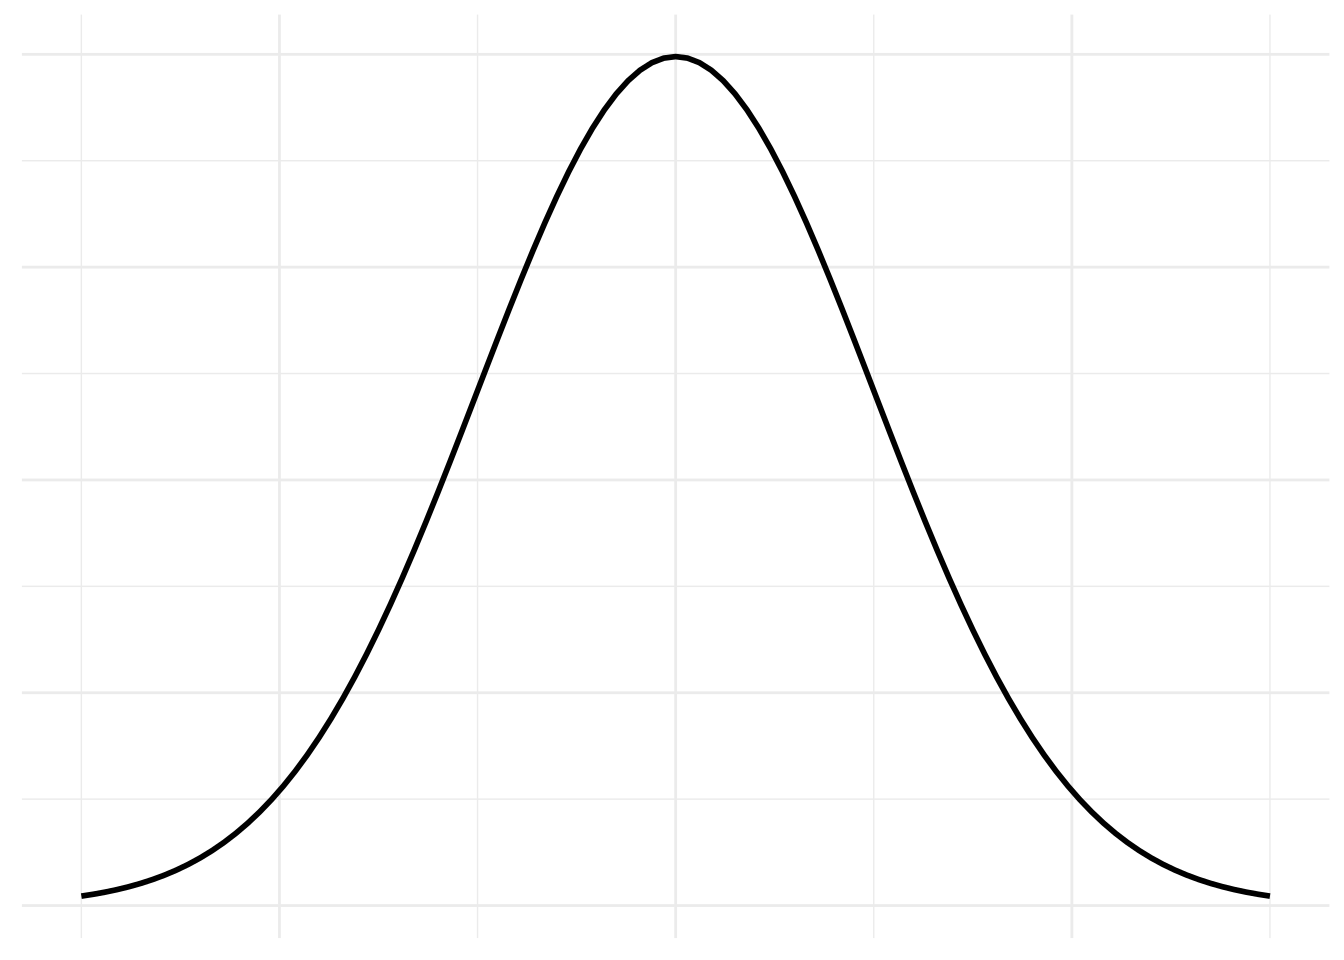
\includegraphics{Introduccion_Datos_files/figure-latex/unnamed-chunk-53-1.pdf}

Dos medidas comunmente utilizadas son la asimetría y la curtosis. La
\textbf{kurtosis} mide que tan coludas son las distribuciones con
respecto a la normal. El 0 representa una distribución normal. Valores
positivos son distribuciones más coludas (con más valores extremos) y
valores negativos distribuciones menos coludas.

\begin{Shaded}
\begin{Highlighting}[]
\NormalTok{knitr}\OperatorTok{::}\KeywordTok{include_graphics}\NormalTok{(}\StringTok{"./img/1008px-Standard_symmetric_pdfs.png"}\NormalTok{)}
\end{Highlighting}
\end{Shaded}

\begin{center}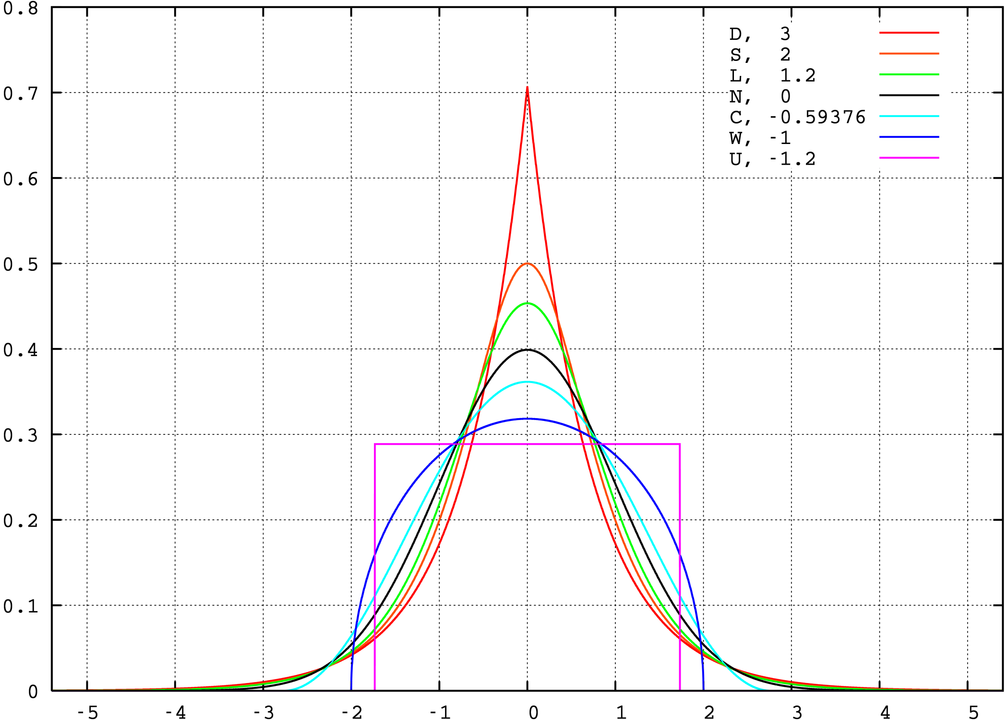
\includegraphics[width=0.75\linewidth]{./img/1008px-Standard_symmetric_pdfs} \end{center}

\begin{itemize}
\tightlist
\item
  Un índice entre -0.5 y 0.5 indica que la distribución es mesocúrtica.
\item
  Un índice mayor a 0.5 insdica que la distribución es leptocúrtica
\item
  Un índice menor a -0.5 indica que la distribución es platicúrtica
\end{itemize}

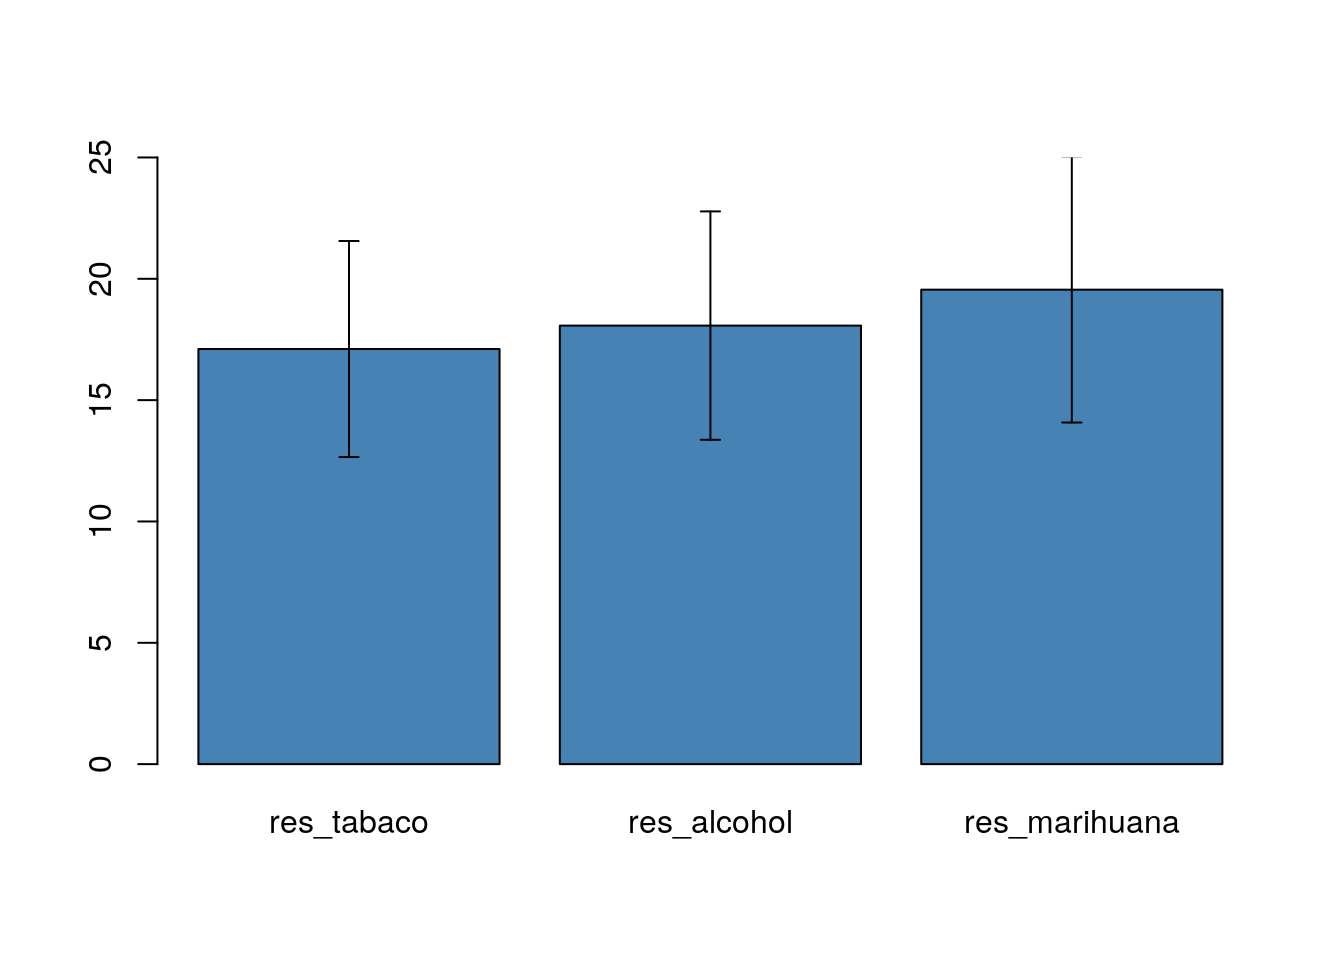
\includegraphics{Introduccion_Datos_files/figure-latex/unnamed-chunk-55-1.pdf}

\section{Estandarización}\label{estandarizacion}

La estandarización mediante los procesos de \textbf{centrado} y
\textbf{escalado} de los datos. Para centrar los datos, les restamos la
media. Para escalarlos, los dividimos por su desvío estándar.

\begin{Shaded}
\begin{Highlighting}[]
\NormalTok{## Seleccionamos la edad y la guardamos en una nueva variable}
\NormalTok{edad <-}\StringTok{ }\NormalTok{enprecosp}\OperatorTok{$}\NormalTok{BHCH05}

\NormalTok{## Centramos}
\NormalTok{edad_centrada <-}\StringTok{ }\NormalTok{edad }\OperatorTok{-}\StringTok{ }\KeywordTok{mean}\NormalTok{(edad)}

\NormalTok{## Escalamos}
\NormalTok{edad_estandarizada <-}\StringTok{ }\NormalTok{edad_centrada }\OperatorTok{/}\StringTok{ }\KeywordTok{sd}\NormalTok{(edad)}

\KeywordTok{head}\NormalTok{(edad)}
\end{Highlighting}
\end{Shaded}

\begin{verbatim}
## [1] 16 59 65 39 19 55
\end{verbatim}

\begin{Shaded}
\begin{Highlighting}[]
\KeywordTok{head}\NormalTok{(edad_estandarizada)}
\end{Highlighting}
\end{Shaded}

\begin{verbatim}
## [1] -1.61510952  1.49337797  1.92712041  0.04756984 -1.39823830  1.20421634
\end{verbatim}

Los puntajes estandarizados, también llamados \textbf{puntajes z}, son
adimensionales. Esa transformación es útil para comparar a los
individuos con su grupo de referencia, y detectar, por ejemplo, valores
extremos. Al ser una medida relativa, también nos sirve para comparar a
un individuo en diferentes variables.\\
Veremos posteriormente que, en las distribuciones normales,
aproximadamente el 95\% de los casos se encuentra entre -2 y 2 desvíos
estandar. Por lo tanto, encontrar individuos con puntajes z mayores a 2
o menores a -2 nos indica que son más bien casos atípicos.

\chapter{Gráficos de Resumen}\label{graficos-de-resumen}

\section{Gráficos de barras}\label{graficos-de-barras}

Los gráficos de barras también sirven para graficar las medias. También
podemos agregar las

\begin{Shaded}
\begin{Highlighting}[]
\KeywordTok{library}\NormalTok{(Hmisc)}
\end{Highlighting}
\end{Shaded}

\begin{Shaded}
\begin{Highlighting}[]
\NormalTok{## Seleccionamos las variables de edad de inicio de consumo}
\NormalTok{## para tabaco, alcohol y marihuana}
\NormalTok{edad_tabaco <-}\StringTok{ }\NormalTok{enprecosp}\OperatorTok{$}\NormalTok{BITA03[enprecosp}\OperatorTok{$}\NormalTok{BITA03 }\OperatorTok{!=}\StringTok{ }\DecValTok{99}\NormalTok{]}
\NormalTok{edad_alcohol <-}\StringTok{ }\NormalTok{enprecosp}\OperatorTok{$}\NormalTok{BIBA03[enprecosp}\OperatorTok{$}\NormalTok{BIBA03 }\OperatorTok{!=}\StringTok{ }\DecValTok{99}\NormalTok{]}
\NormalTok{edad_marihuana <-}\StringTok{ }\NormalTok{enprecosp}\OperatorTok{$}\NormalTok{BIMA03[enprecosp}\OperatorTok{$}\NormalTok{BIMA03 }\OperatorTok{!=}\StringTok{ }\DecValTok{99}\NormalTok{]}

\NormalTok{## Calculamos la media y el desvío estandar}
\NormalTok{res_tabaco <-}\StringTok{ }\KeywordTok{c}\NormalTok{(}\KeywordTok{mean}\NormalTok{(edad_tabaco, }\DataTypeTok{na.rm =} \OtherTok{TRUE}\NormalTok{), }\KeywordTok{sd}\NormalTok{(edad_tabaco, }\DataTypeTok{na.rm =} \OtherTok{TRUE}\NormalTok{))}
\NormalTok{res_alcohol <-}\StringTok{ }\KeywordTok{c}\NormalTok{(}\KeywordTok{mean}\NormalTok{(edad_alcohol, }\DataTypeTok{na.rm =} \OtherTok{TRUE}\NormalTok{), }\KeywordTok{sd}\NormalTok{(edad_alcohol, }\DataTypeTok{na.rm =} \OtherTok{TRUE}\NormalTok{))}
\NormalTok{res_marihuana <-}\StringTok{ }\KeywordTok{c}\NormalTok{(}\KeywordTok{mean}\NormalTok{(edad_marihuana, }\DataTypeTok{na.rm =} \OtherTok{TRUE}\NormalTok{), }\KeywordTok{sd}\NormalTok{(edad_marihuana, }\DataTypeTok{na.rm =} \OtherTok{TRUE}\NormalTok{))}

\NormalTok{## Construimos una matriz con los resultados}
\NormalTok{m <-}\StringTok{ }\KeywordTok{cbind}\NormalTok{(res_tabaco, res_alcohol, res_marihuana)}

\NormalTok{## Armamos el gráfico de barras}
\NormalTok{b <-}\StringTok{ }\KeywordTok{barplot}\NormalTok{(m[}\DecValTok{1}\NormalTok{,], }\DataTypeTok{ylim =} \KeywordTok{c}\NormalTok{(}\DecValTok{0}\NormalTok{, }\DecValTok{25}\NormalTok{), }\DataTypeTok{col =} \StringTok{"steelblue"}\NormalTok{)}
\CommentTok{# errbar(colnames(m), m[1,], m[1,] + m[2,], m[1,] - m[2,])}
\KeywordTok{arrows}\NormalTok{(b, m[}\DecValTok{1}\NormalTok{,] }\OperatorTok{-}\StringTok{ }\NormalTok{m[}\DecValTok{2}\NormalTok{,], b, m[}\DecValTok{1}\NormalTok{,] }\OperatorTok{+}\StringTok{ }\NormalTok{m[}\DecValTok{2}\NormalTok{,], }\DataTypeTok{length=}\FloatTok{0.05}\NormalTok{, }\DataTypeTok{angle=}\DecValTok{90}\NormalTok{, }\DataTypeTok{code=}\DecValTok{3}\NormalTok{)}
\end{Highlighting}
\end{Shaded}

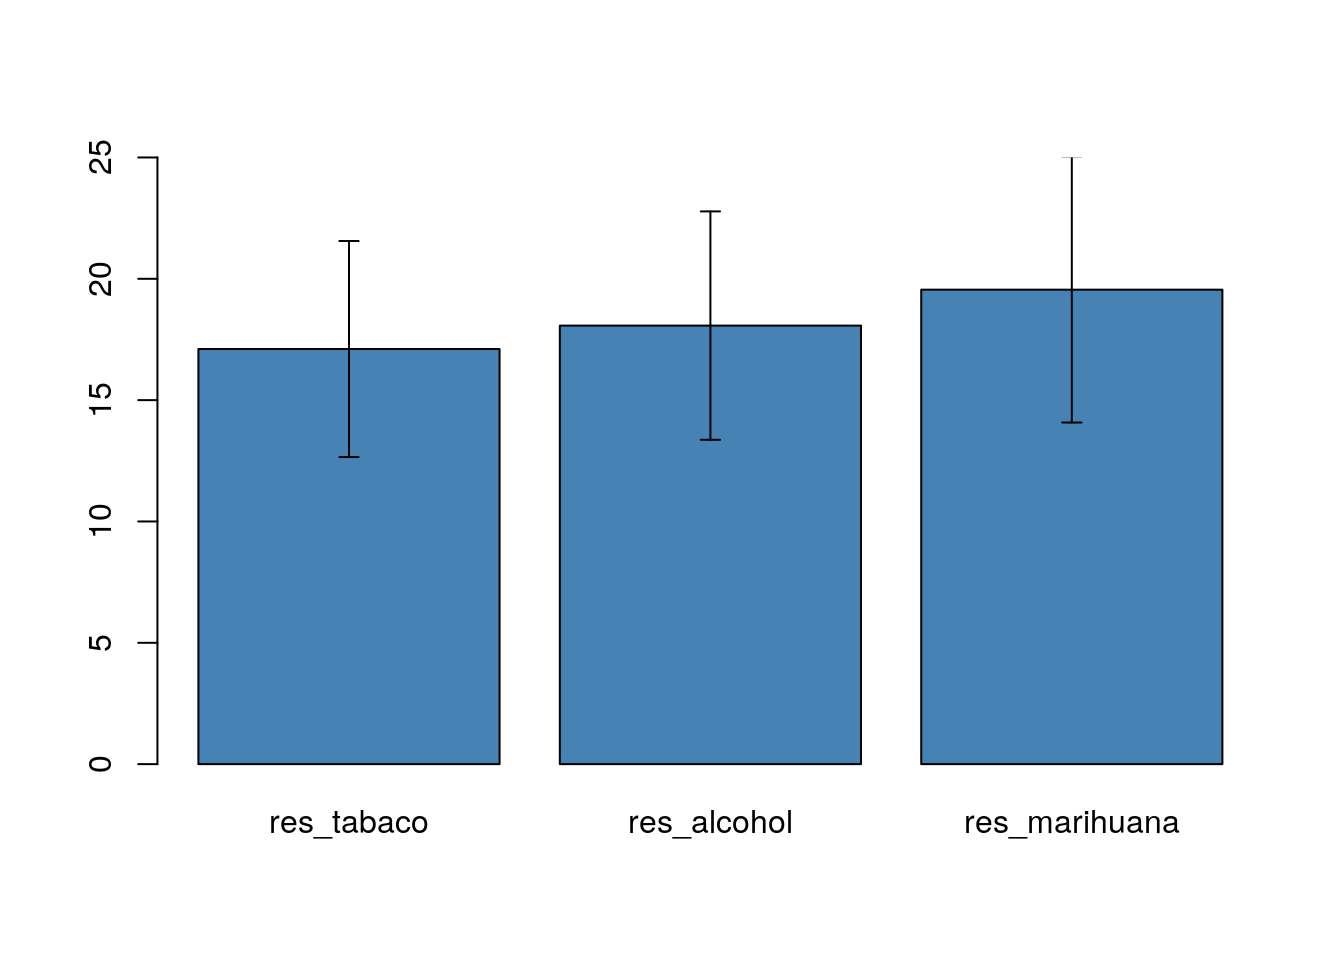
\includegraphics{Introduccion_Datos_files/figure-latex/unnamed-chunk-59-1.pdf}

\begin{Shaded}
\begin{Highlighting}[]
\CommentTok{# x <- factor(c("tabaco", "alcohol", "marihuana"))}
\CommentTok{# medias <- c(mean(edad_tabaco, na.rm = TRUE),}
\CommentTok{#             mean(edad_alcohol, na.rm = TRUE),}
\CommentTok{#             mean(edad_alcohol, na.rm = TRUE))}
\CommentTok{# sd <- c(sd(edad_tabaco, na.rm = TRUE),}
\CommentTok{#         sd(edad_alcohol, na.rm = TRUE),}
\CommentTok{#         sd(edad_alcohol, na.rm = TRUE))}
\CommentTok{# }
\CommentTok{# barplot(height = medias, width = 1, col = "steelblue")}
\end{Highlighting}
\end{Shaded}

\section{Gráficos de caja}\label{graficos-de-caja}

\begin{Shaded}
\begin{Highlighting}[]
\KeywordTok{boxplot}\NormalTok{(}\KeywordTok{list}\NormalTok{(edad_tabaco, edad_alcohol, edad_marihuana),}
        \DataTypeTok{names =} \KeywordTok{c}\NormalTok{(}\StringTok{"tabaco"}\NormalTok{, }\StringTok{"alcohol"}\NormalTok{, }\StringTok{"marihuana"}\NormalTok{),}
        \DataTypeTok{col =} \StringTok{"tomato"}\NormalTok{,}
        \DataTypeTok{pch =} \DecValTok{16}\NormalTok{)}
\end{Highlighting}
\end{Shaded}

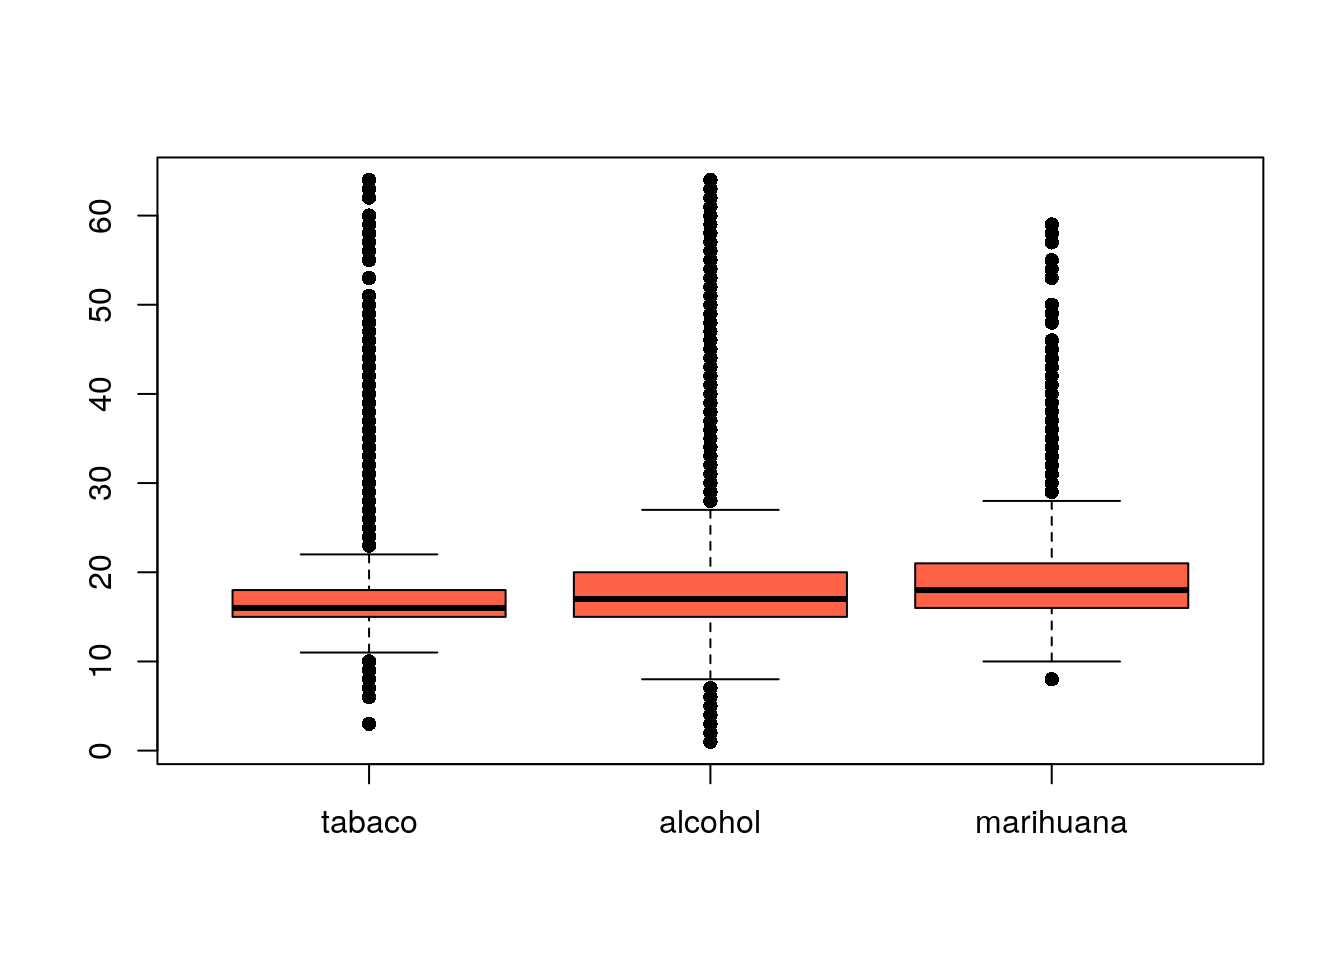
\includegraphics{Introduccion_Datos_files/figure-latex/unnamed-chunk-60-1.pdf}

\begin{verbatim}

Attaching package: 'dplyr'
\end{verbatim}

\begin{verbatim}
The following object is masked from 'package:kableExtra':

    group_rows
\end{verbatim}

\begin{verbatim}
The following objects are masked from 'package:Hmisc':

    src, summarize
\end{verbatim}

\begin{verbatim}
The following objects are masked from 'package:stats':

    filter, lag
\end{verbatim}

\begin{verbatim}
The following objects are masked from 'package:base':

    intersect, setdiff, setequal, union
\end{verbatim}

\chapter{Relaciones entre variables}\label{relaciones-entre-variables}

Hasta aquí hemos venidos trabjando principalmente con medidas de
resúmenes, tablas y gráficos para variables individuales. Muchas veces
interesa obervar como las variables se comportan conjuntamente. Para
ello, también haremos uso de tablas, gráficos y medidas de resúmenes. En
términos técnicos, lo que nos interesesa es explicar la variabilidad.
Podemos explicar parcialmente la variabilidad de una variable conociendo
los valores de otras variables que estén \textbf{asociadas}. Diremos que
existe \textbf{asociación de variables} cuando la variación de una de
ellas influya en la variación de las otras. Por ejemplo, el peso y la
altura son dos variables que están asociadas. Esperaríamos que las
personas que son más altas sean, en promedio, mas pesadas que aquellas
que son más bajas. Diremos que dos variables son \textbf{independientes}
cuando la variación de una de ellas no afecta la variación de la otra.

\section{Tablas de contingencia}\label{tablas-de-contingencia}

Son llamadas también \textbf{tablas de distribución conjunta},
\textbf{tablas bivariadas} o \textbf{tablas cruzadas}. Permite obervar
la relación entre variables cualitativas. Se representan las categorías
de una variables en las filas, y las categorías de la otra en las
columnas, y se pueden calcular diferentes tipos de frecuencias absolutas
o relativas.

Supongamos que queremos observar la relación entre la prevalencia de
consumo con el riesgo percibido para el consumo frecuente de alcohol
(BIBA14\_02).

\begin{Shaded}
\begin{Highlighting}[]
\NormalTok{## Prevalencia de consumo del último mes y riesgo percibido}
\NormalTok{## Alcohol}
\NormalTok{riesgo_perc <-}\StringTok{ }\KeywordTok{factor}\NormalTok{(enprecosp}\OperatorTok{$}\NormalTok{BIBA14_}\DecValTok{02}\NormalTok{,}
                      \DataTypeTok{labels =} \KeywordTok{c}\NormalTok{(}\StringTok{"Ningún riesgo"}\NormalTok{,}
                                 \StringTok{"Riesgo leve o moderado"}\NormalTok{,}
                                 \StringTok{"Gran riesgo"}\NormalTok{,}
                                 \StringTok{"No sé que riesgo corre"}\NormalTok{))}


\NormalTok{prev_mes <-}\StringTok{ }\KeywordTok{factor}\NormalTok{(enprecosp}\OperatorTok{$}\NormalTok{P1M_BA,}
                \DataTypeTok{labels =} \KeywordTok{c}\NormalTok{(}\StringTok{"Sí"}\NormalTok{,}
                           \StringTok{"No"}\NormalTok{))}

\NormalTok{## Realizamos una tabla de frecuencias absolutas conjunta}
\NormalTok{tc <-}\StringTok{ }\KeywordTok{table}\NormalTok{(riesgo_perc, prev_mes)}
\NormalTok{tc}
\end{Highlighting}
\end{Shaded}

\begin{verbatim}
##                         prev_mes
## riesgo_perc                 Sí    No
##   Ningún riesgo            202    61
##   Riesgo leve o moderado  1701  1139
##   Gran riesgo            14261 16601
##   No sé que riesgo corre   163   215
\end{verbatim}

En estas tablas también se pueden expresas las frecuencias marginales.
Las \textbf{frecuencias marginales} son los totales por fila y por
columna. Se corresponden con las frecuencias univariadas para cada una
de las variables.

\begin{Shaded}
\begin{Highlighting}[]
\NormalTok{## Frecuencias marginales}
\KeywordTok{addmargins}\NormalTok{(tc)}
\end{Highlighting}
\end{Shaded}

\begin{verbatim}
##                         prev_mes
## riesgo_perc                 Sí    No   Sum
##   Ningún riesgo            202    61   263
##   Riesgo leve o moderado  1701  1139  2840
##   Gran riesgo            14261 16601 30862
##   No sé que riesgo corre   163   215   378
##   Sum                    16327 18016 34343
\end{verbatim}

También podemos calcular las frecuencias relativas

\begin{Shaded}
\begin{Highlighting}[]
\NormalTok{## Frecuencias relativas al total}
\NormalTok{tc_tot <-}\StringTok{ }\KeywordTok{prop.table}\NormalTok{(tc)}
\NormalTok{tc_tot <-}\StringTok{ }\KeywordTok{addmargins}\NormalTok{(tc_tot)}

\KeywordTok{format}\NormalTok{(tc_tot, }\DataTypeTok{digits =} \DecValTok{0}\NormalTok{, }\DataTypeTok{nsmall =} \DecValTok{4}\NormalTok{)}
\end{Highlighting}
\end{Shaded}

\begin{verbatim}
##                         prev_mes
## riesgo_perc              Sí       No       Sum     
##   Ningún riesgo          "0.0059" "0.0018" "0.0077"
##   Riesgo leve o moderado "0.0495" "0.0332" "0.0827"
##   Gran riesgo            "0.4153" "0.4834" "0.8986"
##   No sé que riesgo corre "0.0047" "0.0063" "0.0110"
##   Sum                    "0.4754" "0.5246" "1.0000"
\end{verbatim}

\begin{Shaded}
\begin{Highlighting}[]
\NormalTok{## Frecuencias relativas por filas}
\NormalTok{tc_fila <-}\StringTok{ }\KeywordTok{addmargins}\NormalTok{(tc, }\DecValTok{1}\NormalTok{)}
\NormalTok{tc_fila <-}\StringTok{ }\KeywordTok{prop.table}\NormalTok{(tc_fila, }\DecValTok{1}\NormalTok{)}

\KeywordTok{format}\NormalTok{(tc_fila, }\DataTypeTok{digits =} \DecValTok{0}\NormalTok{, }\DataTypeTok{nsmall =} \DecValTok{4}\NormalTok{)}
\end{Highlighting}
\end{Shaded}

\begin{verbatim}
##                         prev_mes
## riesgo_perc              Sí       No      
##   Ningún riesgo          "0.7681" "0.2319"
##   Riesgo leve o moderado "0.5989" "0.4011"
##   Gran riesgo            "0.4621" "0.5379"
##   No sé que riesgo corre "0.4312" "0.5688"
##   Sum                    "0.4754" "0.5246"
\end{verbatim}

\begin{Shaded}
\begin{Highlighting}[]
\NormalTok{## Frecuencias relativas por columna}
\NormalTok{tc_col <-}\StringTok{ }\KeywordTok{addmargins}\NormalTok{(tc, }\DecValTok{2}\NormalTok{)}
\NormalTok{tc_col <-}\StringTok{ }\KeywordTok{prop.table}\NormalTok{(tc_col, }\DecValTok{2}\NormalTok{)}

\KeywordTok{format}\NormalTok{(tc_col, }\DataTypeTok{digits =} \DecValTok{0}\NormalTok{, }\DataTypeTok{nsmall =} \DecValTok{4}\NormalTok{)}
\end{Highlighting}
\end{Shaded}

\begin{verbatim}
##                         prev_mes
## riesgo_perc              Sí       No       Sum     
##   Ningún riesgo          "0.0124" "0.0034" "0.0077"
##   Riesgo leve o moderado "0.1042" "0.0632" "0.0827"
##   Gran riesgo            "0.8735" "0.9215" "0.8986"
##   No sé que riesgo corre "0.0100" "0.0119" "0.0110"
\end{verbatim}

\section{Riesgo relativo}\label{riesgo-relativo}

\begin{longtable}[]{@{}llll@{}}
\toprule
& Enfermo & Saludable & Total\tabularnewline
\midrule
\endhead
Expuesto & \(D_e\) & \(H_e\) & \(N_e\)\tabularnewline
No Expuesto & \(D_n\) & \(H_n\) & \(N_n\)\tabularnewline
\bottomrule
\end{longtable}

\[
RR = \frac{D_e/N_e}{D_n/N_n}
\]

\section{Odds ratio}\label{odds-ratio}

\[
OR = \frac{D_e/H_e}{D_n/H_n}
\]

\section{Intensidad de la asociación}\label{intensidad-de-la-asociacion}

Las medidas de asociación nos permiten evaluar el grado o intensidad de
la relación entre las variables.

\subsection{Q de Kendall - Yule}\label{q-de-kendall---yule}

El Q de Kendall-Yule es una medida de intensidad de asociación para
variables dicotómicas. Supongamos que tenemos la siguiente tabla de
doble entrada:

\begin{table}[H]
\centering
\begin{tabular}{l|l|l|l}
\hline
  & Sí & No & Total\\
\hline
Positiva & a & b & a+b\\
\hline
Negativa & c & d & c+d\\
\hline
Total & a+c & b+d & n\\
\hline
\end{tabular}
\end{table}

El coeficiente de Q es:

\[
Q = \frac{ad - bc}{ad + bc}
\]

Evaluemos si el sexo está relacionado con la prevalencia mensual de
consumo de alcohol.

\begin{Shaded}
\begin{Highlighting}[]
\NormalTok{sexo <-}\StringTok{ }\KeywordTok{factor}\NormalTok{(enprecosp}\OperatorTok{$}\NormalTok{BHCH04J,}
                    \DataTypeTok{labels =} \KeywordTok{c}\NormalTok{(}\StringTok{"Varón",}
\StringTok{                               "}\NormalTok{Mujer}\StringTok{"))}

\StringTok{prev_alcohol <- factor(enprecosp$P1M_BA,}
\StringTok{                    labels = c("}\NormalTok{Sí}\StringTok{",}
\StringTok{                               "}\NormalTok{No}\StringTok{"))}

\StringTok{tc <- table(sexo, prev_alcohol)}

\StringTok{tc}
\end{Highlighting}
\end{Shaded}

\begin{verbatim}
##        prev_alcohol
## sexo       Sí    No
##   Varón 11378 11434
##   Mujer  4949  6582
\end{verbatim}

\begin{Shaded}
\begin{Highlighting}[]
\NormalTok{## Veamos el grado de asociación}
\NormalTok{a <-}\StringTok{ }\NormalTok{tc[}\DecValTok{1}\NormalTok{,}\DecValTok{1}\NormalTok{]}
\NormalTok{b <-}\StringTok{ }\NormalTok{tc[}\DecValTok{1}\NormalTok{,}\DecValTok{2}\NormalTok{]}
\NormalTok{c <-}\StringTok{ }\NormalTok{tc[}\DecValTok{2}\NormalTok{,}\DecValTok{1}\NormalTok{]}
\NormalTok{d <-}\StringTok{ }\NormalTok{tc[}\DecValTok{2}\NormalTok{,}\DecValTok{2}\NormalTok{]}


\NormalTok{## Calculamos el coeficiente Q de Kendall-Yule}
\NormalTok{Q <-}\StringTok{ }\NormalTok{(a}\OperatorTok{*}\NormalTok{d}\OperatorTok{-}\NormalTok{b}\OperatorTok{*}\NormalTok{c)}\OperatorTok{/}\NormalTok{(a}\OperatorTok{*}\NormalTok{d}\OperatorTok{+}\NormalTok{b}\OperatorTok{*}\NormalTok{c)}
\NormalTok{Q}
\end{Highlighting}
\end{Shaded}

\begin{verbatim}
## [1] 0.1392118
\end{verbatim}

\subsection{\texorpdfstring{Chi cuadrado
(\(\chi^2\))}{Chi cuadrado (\textbackslash{}chi\^{}2)}}\label{chi-cuadrado-chi2}

\begin{Shaded}
\begin{Highlighting}[]
\NormalTok{## Riesgo leve percibido}
\NormalTok{## En su opinión, ¿cuál cree usted que es el riesgo que}
\NormalTok{## corre una persona que toma bebidas alcohólicas de vez}
\NormalTok{## en cuando}

\NormalTok{riesgo_perc <-}\StringTok{ }\KeywordTok{factor}\NormalTok{(enprecosp}\OperatorTok{$}\NormalTok{BIBA14_}\DecValTok{01}\NormalTok{,}
                      \DataTypeTok{labels =} \KeywordTok{c}\NormalTok{(}\StringTok{"Ningún riesgo"}\NormalTok{,}
                                 \StringTok{"Riesgo leve o moderado"}\NormalTok{,}
                                 \StringTok{"Gran riesgo"}\NormalTok{,}
                                 \StringTok{"No sé qué riesgo"}\NormalTok{))}

\CommentTok{# prop.table(table(riesgo_perc))}

\NormalTok{prev_alcohol <-}\StringTok{ }\KeywordTok{factor}\NormalTok{(enprecosp}\OperatorTok{$}\NormalTok{P1M_BA,}
                    \DataTypeTok{labels =} \KeywordTok{c}\NormalTok{(}\StringTok{"Sí"}\NormalTok{,}
                               \StringTok{"No"}\NormalTok{))}

\NormalTok{tc <-}\StringTok{ }\KeywordTok{table}\NormalTok{(riesgo_perc, prev_alcohol)}

\NormalTok{## Calculamos las frecuencias esperadas y observadas}
\NormalTok{chi <-}\StringTok{ }\KeywordTok{chisq.test}\NormalTok{(tc)}
\NormalTok{chi}\OperatorTok{$}\NormalTok{observed}
\end{Highlighting}
\end{Shaded}

\begin{verbatim}
##                         prev_alcohol
## riesgo_perc                Sí   No
##   Ningún riesgo          4153 2813
##   Riesgo leve o moderado 7432 7309
##   Gran riesgo            4549 7622
##   No sé qué riesgo        193  272
\end{verbatim}

\begin{Shaded}
\begin{Highlighting}[]
\NormalTok{chi}\OperatorTok{$}\NormalTok{expected}
\end{Highlighting}
\end{Shaded}

\begin{verbatim}
##                         prev_alcohol
## riesgo_perc                     Sí        No
##   Ningún riesgo          3311.7049 3654.2951
##   Riesgo leve o moderado 7008.0164 7732.9836
##   Gran riesgo            5786.2131 6384.7869
##   No sé qué riesgo        221.0656  243.9344
\end{verbatim}

\begin{Shaded}
\begin{Highlighting}[]
\NormalTok{chi_val <-}\StringTok{ }\NormalTok{chi}\OperatorTok{$}\NormalTok{statistic; chi_val}
\end{Highlighting}
\end{Shaded}

\begin{verbatim}
## X-squared 
##   967.376
\end{verbatim}

\section{\texorpdfstring{Coeficiente Phi de Pearson-Yule
(\(\varphi\))}{Coeficiente Phi de Pearson-Yule (\textbackslash{}varphi)}}\label{coeficiente-phi-de-pearson-yule-varphi}

\[
\varphi = \sqrt{\frac{\chi^2}{n}}
\]

\begin{Shaded}
\begin{Highlighting}[]
\NormalTok{sexo <-}\StringTok{ }\KeywordTok{factor}\NormalTok{(enprecosp}\OperatorTok{$}\NormalTok{BHCH04J,}
                    \DataTypeTok{labels =} \KeywordTok{c}\NormalTok{(}\StringTok{"Varón",}
\StringTok{                               "}\NormalTok{Mujer}\StringTok{"))}

\StringTok{prev_alcohol <- factor(enprecosp$P1M_BA,}
\StringTok{                    labels = c("}\NormalTok{Sí}\StringTok{",}
\StringTok{                               "}\NormalTok{No}\StringTok{"))}

\StringTok{tc <- table(sexo, prev_alcohol)}

\StringTok{chi <- chisq.test(tc)}
\StringTok{chi_val <- chi$statistic}

\StringTok{n <- sum(tc)}
\StringTok{phi <- sqrt(chi_val/n)}
\end{Highlighting}
\end{Shaded}

\subsection{Coeficiente de contingencia C de
Pearson}\label{coeficiente-de-contingencia-c-de-pearson}

Mide el grado de asociación en tablas de contingencia con más de dos
categorías.

\[
C = \sqrt{\frac{\chi^2}{\chi^2 + n}}
\]

Va de 0 a 1 y se compara con un C máximo:

\[
C_{max} = \sqrt{\frac{min(f, c) - 1}{min(f, c)}}
\] Donde: \(f\) es el número de filas \(g\) es el número de columnas

\begin{Shaded}
\begin{Highlighting}[]
\NormalTok{## Riesgo leve percibido}
\NormalTok{## En su opinión, ¿cuál cree usted que es el riesgo que}
\NormalTok{## corre una persona que toma bebidas alcohólicas de vez}
\NormalTok{## en cuando}

\NormalTok{riesgo_perc <-}\StringTok{ }\KeywordTok{factor}\NormalTok{(enprecosp}\OperatorTok{$}\NormalTok{BIBA14_}\DecValTok{01}\NormalTok{,}
                      \DataTypeTok{labels =} \KeywordTok{c}\NormalTok{(}\StringTok{"Ningún riesgo"}\NormalTok{,}
                                 \StringTok{"Riesgo leve o moderado"}\NormalTok{,}
                                 \StringTok{"Gran riesgo"}\NormalTok{,}
                                 \StringTok{"No sé qué riesgo"}\NormalTok{))}

\CommentTok{# prop.table(table(riesgo_perc))}

\NormalTok{prev_alcohol <-}\StringTok{ }\KeywordTok{factor}\NormalTok{(enprecosp}\OperatorTok{$}\NormalTok{P1M_BA,}
                    \DataTypeTok{labels =} \KeywordTok{c}\NormalTok{(}\StringTok{"Sí"}\NormalTok{,}
                               \StringTok{"No"}\NormalTok{))}

\NormalTok{tc <-}\StringTok{ }\KeywordTok{table}\NormalTok{(riesgo_perc, prev_alcohol)}

\NormalTok{## Calculamos las frecuencias esperadas y observadas}
\NormalTok{chi <-}\StringTok{ }\KeywordTok{chisq.test}\NormalTok{(tc)}
\NormalTok{chi}\OperatorTok{$}\NormalTok{observed}
\end{Highlighting}
\end{Shaded}

\begin{verbatim}
##                         prev_alcohol
## riesgo_perc                Sí   No
##   Ningún riesgo          4153 2813
##   Riesgo leve o moderado 7432 7309
##   Gran riesgo            4549 7622
##   No sé qué riesgo        193  272
\end{verbatim}

\begin{Shaded}
\begin{Highlighting}[]
\NormalTok{chi}\OperatorTok{$}\NormalTok{expected}
\end{Highlighting}
\end{Shaded}

\begin{verbatim}
##                         prev_alcohol
## riesgo_perc                     Sí        No
##   Ningún riesgo          3311.7049 3654.2951
##   Riesgo leve o moderado 7008.0164 7732.9836
##   Gran riesgo            5786.2131 6384.7869
##   No sé qué riesgo        221.0656  243.9344
\end{verbatim}

\begin{Shaded}
\begin{Highlighting}[]
\NormalTok{chi_val <-}\StringTok{ }\NormalTok{chi}\OperatorTok{$}\NormalTok{statistic; chi_val}
\end{Highlighting}
\end{Shaded}

\begin{verbatim}
## X-squared 
##   967.376
\end{verbatim}

\begin{Shaded}
\begin{Highlighting}[]
\NormalTok{## Calculamos el C de Pearson}
\NormalTok{f <-}\StringTok{ }\KeywordTok{nrow}\NormalTok{(tc)}
\NormalTok{c <-}\StringTok{ }\KeywordTok{ncol}\NormalTok{(tc)}
\NormalTok{n <-}\StringTok{ }\KeywordTok{sum}\NormalTok{(tc)}
\NormalTok{C <-}\StringTok{ }\KeywordTok{sqrt}\NormalTok{(chi_val}\OperatorTok{/}\NormalTok{(chi_val }\OperatorTok{+}\StringTok{ }\NormalTok{n)); C}
\end{Highlighting}
\end{Shaded}

\begin{verbatim}
## X-squared 
## 0.1655185
\end{verbatim}

\begin{Shaded}
\begin{Highlighting}[]
\NormalTok{Cmax <-}\StringTok{ }\KeywordTok{sqrt}\NormalTok{((}\KeywordTok{min}\NormalTok{(f, c) }\OperatorTok{-}\StringTok{ }\DecValTok{1}\NormalTok{) }\OperatorTok{/}\StringTok{ }\KeywordTok{min}\NormalTok{(f, c)); Cmax}
\end{Highlighting}
\end{Shaded}

\begin{verbatim}
## [1] 0.7071068
\end{verbatim}

\subsection{Coeficiente V de Cramer}\label{coeficiente-v-de-cramer}

\[
V = \sqrt{\frac{\chi^2}{n * min(f - 1, c-1)}}
\]

\begin{Shaded}
\begin{Highlighting}[]
\NormalTok{V <-}\StringTok{ }\KeywordTok{sqrt}\NormalTok{(chi_val}\OperatorTok{/}\NormalTok{(n }\OperatorTok{*}\StringTok{ }\KeywordTok{min}\NormalTok{(}\KeywordTok{ncol}\NormalTok{(tc), }\KeywordTok{nrow}\NormalTok{(tc))))}
\end{Highlighting}
\end{Shaded}

\bibliography{book.bib,packages.bib}


\end{document}
